% Options for packages loaded elsewhere
\PassOptionsToPackage{unicode}{hyperref}
\PassOptionsToPackage{hyphens}{url}
%
\documentclass[
  man,mask]{apa6}
\usepackage{amsmath,amssymb}
\usepackage{iftex}
\ifPDFTeX
  \usepackage[T1]{fontenc}
  \usepackage[utf8]{inputenc}
  \usepackage{textcomp} % provide euro and other symbols
\else % if luatex or xetex
  \usepackage{unicode-math} % this also loads fontspec
  \defaultfontfeatures{Scale=MatchLowercase}
  \defaultfontfeatures[\rmfamily]{Ligatures=TeX,Scale=1}
\fi
\usepackage{lmodern}
\ifPDFTeX\else
  % xetex/luatex font selection
\fi
% Use upquote if available, for straight quotes in verbatim environments
\IfFileExists{upquote.sty}{\usepackage{upquote}}{}
\IfFileExists{microtype.sty}{% use microtype if available
  \usepackage[]{microtype}
  \UseMicrotypeSet[protrusion]{basicmath} % disable protrusion for tt fonts
}{}
\makeatletter
\@ifundefined{KOMAClassName}{% if non-KOMA class
  \IfFileExists{parskip.sty}{%
    \usepackage{parskip}
  }{% else
    \setlength{\parindent}{0pt}
    \setlength{\parskip}{6pt plus 2pt minus 1pt}}
}{% if KOMA class
  \KOMAoptions{parskip=half}}
\makeatother
\usepackage{xcolor}
\usepackage{graphicx}
\makeatletter
\def\maxwidth{\ifdim\Gin@nat@width>\linewidth\linewidth\else\Gin@nat@width\fi}
\def\maxheight{\ifdim\Gin@nat@height>\textheight\textheight\else\Gin@nat@height\fi}
\makeatother
% Scale images if necessary, so that they will not overflow the page
% margins by default, and it is still possible to overwrite the defaults
% using explicit options in \includegraphics[width, height, ...]{}
\setkeys{Gin}{width=\maxwidth,height=\maxheight,keepaspectratio}
% Set default figure placement to htbp
\makeatletter
\def\fps@figure{htbp}
\makeatother
\setlength{\emergencystretch}{3em} % prevent overfull lines
\providecommand{\tightlist}{%
  \setlength{\itemsep}{0pt}\setlength{\parskip}{0pt}}
\setcounter{secnumdepth}{-\maxdimen} % remove section numbering
% Make \paragraph and \subparagraph free-standing
\makeatletter
\ifx\paragraph\undefined\else
  \let\oldparagraph\paragraph
  \renewcommand{\paragraph}{
    \@ifstar
      \xxxParagraphStar
      \xxxParagraphNoStar
  }
  \newcommand{\xxxParagraphStar}[1]{\oldparagraph*{#1}\mbox{}}
  \newcommand{\xxxParagraphNoStar}[1]{\oldparagraph{#1}\mbox{}}
\fi
\ifx\subparagraph\undefined\else
  \let\oldsubparagraph\subparagraph
  \renewcommand{\subparagraph}{
    \@ifstar
      \xxxSubParagraphStar
      \xxxSubParagraphNoStar
  }
  \newcommand{\xxxSubParagraphStar}[1]{\oldsubparagraph*{#1}\mbox{}}
  \newcommand{\xxxSubParagraphNoStar}[1]{\oldsubparagraph{#1}\mbox{}}
\fi
\makeatother
% definitions for citeproc citations
\NewDocumentCommand\citeproctext{}{}
\NewDocumentCommand\citeproc{mm}{%
  \begingroup\def\citeproctext{#2}\cite{#1}\endgroup}
\makeatletter
 % allow citations to break across lines
 \let\@cite@ofmt\@firstofone
 % avoid brackets around text for \cite:
 \def\@biblabel#1{}
 \def\@cite#1#2{{#1\if@tempswa , #2\fi}}
\makeatother
\newlength{\cslhangindent}
\setlength{\cslhangindent}{1.5em}
\newlength{\csllabelwidth}
\setlength{\csllabelwidth}{3em}
\newenvironment{CSLReferences}[2] % #1 hanging-indent, #2 entry-spacing
 {\begin{list}{}{%
  \setlength{\itemindent}{0pt}
  \setlength{\leftmargin}{0pt}
  \setlength{\parsep}{0pt}
  % turn on hanging indent if param 1 is 1
  \ifodd #1
   \setlength{\leftmargin}{\cslhangindent}
   \setlength{\itemindent}{-1\cslhangindent}
  \fi
  % set entry spacing
  \setlength{\itemsep}{#2\baselineskip}}}
 {\end{list}}
\usepackage{calc}
\newcommand{\CSLBlock}[1]{\hfill\break\parbox[t]{\linewidth}{\strut\ignorespaces#1\strut}}
\newcommand{\CSLLeftMargin}[1]{\parbox[t]{\csllabelwidth}{\strut#1\strut}}
\newcommand{\CSLRightInline}[1]{\parbox[t]{\linewidth - \csllabelwidth}{\strut#1\strut}}
\newcommand{\CSLIndent}[1]{\hspace{\cslhangindent}#1}
\ifLuaTeX
\usepackage[bidi=basic]{babel}
\else
\usepackage[bidi=default]{babel}
\fi
\babelprovide[main,import]{english}
% get rid of language-specific shorthands (see #6817):
\let\LanguageShortHands\languageshorthands
\def\languageshorthands#1{}
% Manuscript styling
\usepackage{upgreek}
\captionsetup{font=singlespacing,justification=justified}

% Table formatting
\usepackage{longtable}
\usepackage{lscape}
% \usepackage[counterclockwise]{rotating}   % Landscape page setup for large tables
\usepackage{multirow}		% Table styling
\usepackage{tabularx}		% Control Column width
\usepackage[flushleft]{threeparttable}	% Allows for three part tables with a specified notes section
\usepackage{threeparttablex}            % Lets threeparttable work with longtable

% Create new environments so endfloat can handle them
% \newenvironment{ltable}
%   {\begin{landscape}\centering\begin{threeparttable}}
%   {\end{threeparttable}\end{landscape}}
\newenvironment{lltable}{\begin{landscape}\centering\begin{ThreePartTable}}{\end{ThreePartTable}\end{landscape}}

% Enables adjusting longtable caption width to table width
% Solution found at http://golatex.de/longtable-mit-caption-so-breit-wie-die-tabelle-t15767.html
\makeatletter
\newcommand\LastLTentrywidth{1em}
\newlength\longtablewidth
\setlength{\longtablewidth}{1in}
\newcommand{\getlongtablewidth}{\begingroup \ifcsname LT@\roman{LT@tables}\endcsname \global\longtablewidth=0pt \renewcommand{\LT@entry}[2]{\global\advance\longtablewidth by ##2\relax\gdef\LastLTentrywidth{##2}}\@nameuse{LT@\roman{LT@tables}} \fi \endgroup}

% \setlength{\parindent}{0.5in}
% \setlength{\parskip}{0pt plus 0pt minus 0pt}

% Overwrite redefinition of paragraph and subparagraph by the default LaTeX template
% See https://github.com/crsh/papaja/issues/292
\makeatletter
\renewcommand{\paragraph}{\@startsection{paragraph}{4}{\parindent}%
  {0\baselineskip \@plus 0.2ex \@minus 0.2ex}%
  {-1em}%
  {\normalfont\normalsize\bfseries\itshape\typesectitle}}

\renewcommand{\subparagraph}[1]{\@startsection{subparagraph}{5}{1em}%
  {0\baselineskip \@plus 0.2ex \@minus 0.2ex}%
  {-\z@\relax}%
  {\normalfont\normalsize\itshape\hspace{\parindent}{#1}\textit{\addperi}}{\relax}}
\makeatother

\makeatletter
\usepackage{etoolbox}
\patchcmd{\maketitle}
  {\section{\normalfont\normalsize\abstractname}}
  {\section*{\normalfont\normalsize\abstractname}}
  {}{\typeout{Failed to patch abstract.}}
\patchcmd{\maketitle}
  {\section{\protect\normalfont{\@title}}}
  {\section*{\protect\normalfont{\@title}}}
  {}{\typeout{Failed to patch title.}}
\makeatother

\usepackage{xpatch}
\makeatletter
\xapptocmd\appendix
  {\xapptocmd\section
    {\addcontentsline{toc}{section}{\appendixname\ifoneappendix\else~\theappendix\fi\\: #1}}
    {}{\InnerPatchFailed}%
  }
{}{\PatchFailed}
\keywords{Latent interaction, UPI, RAPI, 2S-PA}
\DeclareDelayedFloatFlavor{ThreePartTable}{table}
\DeclareDelayedFloatFlavor{lltable}{table}
\DeclareDelayedFloatFlavor*{longtable}{table}
\makeatletter
\renewcommand{\efloat@iwrite}[1]{\immediate\expandafter\protected@write\csname efloat@post#1\endcsname{}}
\makeatother
\usepackage{lineno}

\linenumbers
\usepackage{csquotes}
\ifLuaTeX
  \usepackage{selnolig}  % disable illegal ligatures
\fi
\usepackage{bookmark}
\IfFileExists{xurl.sty}{\usepackage{xurl}}{} % add URL line breaks if available
\urlstyle{same}
\hypersetup{
  pdftitle={Two-Stage Path Analysis with Interaction: An Alternative Method of Modeling Latent Interaction Effects},
  pdflang={en-EN},
  pdfkeywords={Latent interaction, UPI, RAPI, 2S-PA},
  hidelinks,
  pdfcreator={LaTeX via pandoc}}

\title{Two-Stage Path Analysis with Interaction: An Alternative Method of Modeling Latent Interaction Effects}
\author{Gengrui (Jimmy) Zhang\textsuperscript{1}}
\date{}


\shorttitle{2S-PA-Int}

\authornote{

The authors made the following contributions. Gengrui (Jimmy) Zhang: Conceptualization, Writing - Original Draft Preparation, Writing - Review \& Editing.

Correspondence concerning this article should be addressed to Gengrui (Jimmy) Zhang. E-mail: \href{mailto:gengruiz@email.com}{\nolinkurl{gengruiz@email.com}}

}

\affiliation{\vspace{0.5cm}\textsuperscript{1} University of Southhern California}

\abstract{%
Modeling interaction effects within the latent variable modeling framework has become increasingly popular in psychological research as it facilitates exploration of in-depth theory and complex data structure. Comprared to the extensitvely used regression-based approaches assuming error-free variables, latent variable approach is able to account for measurement error and produce estimates with less bias and more accurate standard errors. Through a simulation study, we evaluated and compared three product indicator methods based on structural equation modeling (SEM): Matched-pair Unconstrained Product Indicator (UPI), Reliability-Adjusted Product Indicator (RAPI), and an extended model based on the two-stage path analysis (2S-PA) framework, namely 2S-PA-Int. Our results showed that 2S-PA-Int consistently yielded estimates of interaction effect with low standardized bias, acceptable relative standard error bias, adequate coverage rates, and reasonable root mean square errors. The performance of 2S-PA-Int was comparable to that of matched-pair UPI and RAPI, particularly under conditions of small sample size and low reliability. Given its promising statistical properties and straightforward model specification, 2S-PA-Int emerges as a viable alternative to existing latent interaction methods. Directions for future research on 2S-PA-Int are also discussed.
}



\begin{document}
\maketitle

Social science research increasingly focuses on intricate dynamics of complex phenomena, such as nonlinear and moderation effects, rather than merely simple bivariate relationship. This shift reflects the multifaceted nature of our real world, which seldom conforms to straightforward patterns (Carte \& Russell, 2003; Cunningham \& Ahn, 2019; MacKinnon \& Luecken, 2008). For instance, while earlier studies have established that exercise contributes to weight loss, there is a burgeoning interest in understanding and probing into the underlying mechanisms, such as optimal timing, specific target populations, and the contextual conditions that modulate the effectiveness of exercise in promoting weight loss. Investigations into moderation, or interaction effects, provide critical insights into these inquiries by examining how additional variables, or an ensemble of variables, shape the dynamics between primary variables of interest.

A prevalent approach to modeling moderation is through regression analysis, specifically by incorporating an interaction term, \(XZ\):
\begin{equation}
Y = b_{0} + b_{1}X + b_{2}Z + b_{3}XZ + \epsilon,
\end{equation}
where \(b_{0}\) is the intercept, \(b_{1}\) and \(b_{2}\) are the regression coefficients for \(X\) and \(Z\) respectively, \(b_{3}\) is the coefficient for the interaction term \(XZ\), and \(\epsilon\) is the error term. To maintain consistency with the naming convention used by Marsh et al. (2004), we refer to main effects (i.e., non-interaction effects) as ``first-order effects''. Hence \(X\) and \(Z\) are first-order variables, and \(b_{1}\) and \(b_{2}\) are first-order effects in this case.

Classical regression model typically assumes that variables are measured without error, a premise that can lead to biased parameter estimates when measurement errors are present in empirical research (Bollen, 1989; Carroll et al., 2006; Cohen et al., 2003). This bias is particularly remarkable in the estimation of interaction effects, where measurement error can lead to inflated estimates (Anderson et al., 1996). To mitigate this issue, researchers use latent variables that are inferred and measured by a set of observed indicators within the structural equation modeling (SEM) framework, which can control and accommodate measurement errors in observed indicators (Bollen, 2002). For example, depression is widely measured and assessed using the Center for Epidemiologic Studies Depression (CES-D) scale consisting of 20 items (Radloff, 1977). An expanding body of research has demonstrated that SEM-based moderation models reliably provide more accurate representations of the relationships among latent constructs (Cham et al., 2012; Maslowsky et al., 2015; Mueller, 1997; Steinmetz et al., 2011).

The two-stage path analysis (2S-PA; Lai \& Hsiao, 2022) method models paths or pathway among latent variables through the use of factor scores. Simulation studies have shown its ability to yield parameter estimates with reduced standard error bias, enhanced convergence rates, and improved management of Type I error, particularly in small sample contexts (Lai et al., 2023; Lai \& Hsiao, 2022). Given its promising statistical property, simpler model specification, and easier implementation in widely used software, we extended the 2S-PA method to incorporate latent interaction estimation in this study, and named it 2S-PA-Int. We reviewed two widely used latent interaction models using the product indicator method: Unconstrained Product Indicator with Matched Pairs (Matched-Pair UPI; Marsh et al., 2004) and Reliability-Adjusted Product Indicator (RAPI; Hsiao et al., 2018). Then we conducted a Monte Carlo simulation study to compare their performance with 2S-PA-Int. To proceed, we first introduced a classical model of latent interaction, and then presented UPI, RAPI, and 2S-PA-Int with technical details.

\subsection{A Classical Model of Latent Interaction}\label{a-classical-model-of-latent-interaction}

Kenny and Judd (1984) introduced a seminal structural model for estimating latent interaction effects, particularly in scenarios involving two latent predictors and their interaction term:
\begin{equation}
y = \alpha + \gamma_{x}\xi_{x} + \gamma_{m}\xi_{m} + \gamma_{xm}\xi_{x}\xi_{m} + \zeta,
\end{equation}
where \(\alpha\) is the constant intercept, \(\xi_{x}\) and \(\xi_{m}\) are the first-order latent predictors, and the product \(\xi_{x}\xi_{m}\) defines the interaction effect. Note that \(\xi_{x}\) and \(\xi_{m}\) are allowed to correlate with each other. The disturbance term \(\zeta\) in the model is assumed to follow a normal distribution, \(\zeta \sim N(0, \psi)\), where \(\psi\) denotes the variance of \(\zeta\), accounting for unobserved factors that influence the dependent variable. The coefficients \(\gamma_{x}\) and \(\gamma_{m}\) capture the first-order effects of latent predictors, while \(\gamma_{xm}\) measures the latent interaction effect. The dependent variable \(y\) in this model can be either an observed variable or a latent construct, allowing for flexibility in its application.

The measurement model for the first-order latent predictors, such as \(\xi_{x}\), can be articulated by the following confirmatory factor analysis (CFA) framework:
\begin{equation}
\mathbf{x} = \boldsymbol{\tau_{x}} + \boldsymbol{\lambda_{x}}\xi_{x} + \boldsymbol{\delta_{x}},
\end{equation}
wherein, for each indicator \(i = 1, \ 2, \ ..., \ p_{x}\) associated with the latent predictor \(\xi_{x}\), \(\mathbf{x}\) denotes a \(p_{x} \times 1\) vector of observed first-order indicators (i.e., the indicators of \(\xi_{x}\)). The term \(\boldsymbol{\tau_{x}}\) represents a \(p_{x} \times 1\) vector of constant intercepts, while \(\boldsymbol{\lambda}{x}\) is a \(p_{x} \times 1\) vector of factor loadings, which capture the strength of the relationship between the latent variable \(\xi{x}\) and each of its indicators. The vector \(\boldsymbol{\delta_{x}}\) represents the \(p_{x} \times 1\) vector of measurement errors associated with these indicators. Each measurement error \(\delta_{x_{i}}\) is normally distributed with a mean of zero and a variance of \(\theta_{x_{i}}\). Under the assumption of local independence, which posits that the first-order indicators are uncorrelated with one another when they are indicators of the same latent variable, the variance-covariance matrix of all the indicators' measurement errors is a diagonal matrix, denoted as \(\mathbf{\Theta_{\delta_{x}}} = \text{diag}(\theta_{x_{1}}, \theta_{x_{2}}, ..., \theta_{x_{p}})\). This measurement model, along with its associated parameters, is similarly applicable to the latent predictor \(\xi_{m}\), ensuring consistency in the modeling of both latent variables.

Kenny and Judd's original formulation of model omitted the intercept \(\alpha\), a point subsequently addressed by Jöreskog and Yang (1996), who revised the model under a set of assumptions. The revised latent interaction model is grounded in three primary assumptions related to multivariate normal distribution and independence: (1) The measurement errors of first-order indicators, the first-order latent predictors, and the disturbance term in the structural model are multivariate normal, uncorrelated, and independent to each other (i.e., \(Corr[\delta, \xi] = 0\); \(Corr[\zeta, \xi] = 0\); \(Corr[\delta, \zeta] = 0\), where \(Corr\) denotes the correlation index); (2) All measurement errors are mutually independent and uncorrelated to each other (i.e., \(Corr[\delta_{i}, \delta_{i'}] = 0\) for \(i \neq i'\)); (3) The correlation between the first-order latent predictors, \(Corr[\xi_{x}, \xi_{m}]\), is assumed to be non-zero and is freely estimated. This approach accounts for the fact that the product term \(\xi_{x}\xi_{m}\) may exhibit a non-normal distribution even when \(\xi_{x}\) and \(\xi_{m}\) are themselves normally distributed with means of 0 (Jöreskog \& Yang, 1996).

Algina and Moulder (2001) refined Jöreskog and Yang's (1996) model by introducing the use of mean-centered first-order indicators (e.g., \(x_{i} - \overline{x_{i}}\), where \(\overline{x_{i}}\) represents the mean of \(x_{i}\)) to construct product indicators (PI) that capture the latent interaction term. This enhancement significantly improves the model by rendering parameter estimates more interpretable, facilitating a higher rate of model convergence, and reducing estimation bias (Algina \& Moulder, 2001; Marsh et al., 2004; Moulder \& Algina, 2002). Moreover, the practice of mean-centering first-order indicators effectively mitigates the problem of multicollinearity, thereby more distinctly delineating the contributions of the first-order latent variables and their interactions, as highlighted by Schoemann and Jorgensen (2021).

\subsection{Unconstrained Product Indicator (UPI)}\label{unconstrained-product-indicator-upi}

While Algina and Moulder (2001) significantly improved the model, their approach required complicated nonlinear constraints on parameters of PIs and the interaction term. Constraints in SEM are predefined conditions or restrictions applied to model parameters to ensure model identifiability, theoretical consistency, and interpretability (Kline, 2016). Consider, for example, that \(x_{2}\) and \(m_{2}\) are two first-order indicators of respective latent predictors \(\xi_{x}\) and \(\xi_{m}\), with their corresponding PI formed as \(x_{2}m_{2}\). Then \(x_{2}m_{2}\) can be decomposed using the measurement model of \(x_{2}\) and \(m_{2}\):

\begin{equation}
x_{2}m_{2}= (\lambda_{x_{2}}\xi_{x} + \delta_{x_{2}})(\lambda_{m_{2}}\xi_{m} + \delta_{m_{2}}),
\end{equation}
where \(\lambda\) is the factor loading, \(\xi\) is the first-order latent variable, and \(\delta\) is the error term of first-order indicators. After expanding the equation, it can be shown that the factor loading of this formed PI is a function of first-order indicators' factor loadings, such that \(\lambda_{x_{2}m_{2}} = \lambda_{x_{2}}\lambda_{m_{2}}\). Similarly, the error term can be derived as a function of parameters from first-order indicators: \(\delta_{x_{2}m_{2}} = \lambda_{x_{2}}\xi_{x}\delta_{m_{2}} + \lambda_{m_{2}}\xi_{m}\delta_{x_{2}} + \delta_{x_{2}}\delta_{m_{2}}\). As the number of first-order indicators increases, the model specification becomes overwhelmingly cumbersome due to the resultant nonlinear constraints, which can pose challenges to model convergence.

Marsh et al. (2004) explored methods to eliminate these complex constraints and introduced the innovative Unconstrained Product Indicator (UPI) approach, which simplifies model specification and decreases the likelihood of convergence issues. The structural model of UPI is identical to the model presented in equation (2), with the exception of omitting the intercept \(\alpha\). To illustrate this approach, consider a measurement model where the latent variables \(\xi_{x}\) and \(\xi_{m}\) are each associated with three indicators:

\begin{align}
    \begin{bmatrix}
        x_{1} \\
        x_{2} \\ 
        x_{3}
    \end{bmatrix} =
    \begin{bmatrix}
        \tau_{x_{1}} \\
        \tau_{x_{2}} \\ 
        \tau_{x_{3}}
    \end{bmatrix} +
    \begin{bmatrix}
        \lambda_{x_{1}} \\
        \lambda_{x_{2}} \\ 
        \lambda_{x_{3}}
    \end{bmatrix}
    \begin{bmatrix}
        \xi_{x} \\
    \end{bmatrix} +
    \begin{bmatrix}
        \delta_{x_{1}} \\
        \delta_{x_{2}} \\ 
        \delta_{x_{3}}
    \end{bmatrix},
\end{align}

\begin{align}
    \begin{bmatrix}
        m_{1} \\
        m_{2} \\ 
        m_{3}
    \end{bmatrix} =
    \begin{bmatrix}
        \tau_{m_{1}} \\
        \tau_{m_{2}} \\ 
        \tau_{m_{3}}
    \end{bmatrix} +
    \begin{bmatrix}
        \lambda_{m_{1}} \\
        \lambda_{m_{2}} \\ 
        \lambda_{m_{3}}
    \end{bmatrix}
    \begin{bmatrix}
        \xi_{m} \\
    \end{bmatrix} +
    \begin{bmatrix}
        \delta_{m_{1}} \\
        \delta_{m_{2}} \\ 
        \delta_{m_{3}}
    \end{bmatrix}
\end{align}

Marsh et al. (2004) introduced two methods for specifying UPI: the all-pair UPI and the matched-pair UPI. In the all-pair UPI model, the latent interaction term is represented by all possible pairings of the first-order indicators of \(\xi_{x}\) and \(\xi_{m}\):

\begin{align}
    \begin{bmatrix}
        x_{1}m_{1} \\
        x_{1}m_{2} \\
        x_{1}m_{3} \\ 
        x_{2}m_{1} \\
        ... \\
        x_{3}m_{3}
    \end{bmatrix} = 
    \begin{bmatrix}
        \tau_{x_{1}m_{1}} \\
        \tau_{x_{1}m_{2}} \\ 
        \tau_{x_{1}m_{3}} \\ 
        \tau_{x_{2}m_{1}} \\ 
        ...\\
        \tau_{x_{3}m_{3}} 
    \end{bmatrix} +
    \begin{bmatrix}
        \lambda_{x_{1}m_{1}} \\
        \lambda_{x_{1}m_{2}} \\ 
        \lambda_{x_{1}m_{3}} \\ 
        \lambda_{x_{2}m_{1}} \\ 
        ...\\
        \lambda_{x_{3}m_{3}}
    \end{bmatrix}
    \begin{bmatrix}
        \xi_{x}\xi_{m} \\
    \end{bmatrix} +
    \begin{bmatrix}
        \delta_{x_{1}m_{1}} \\
        \delta_{x_{1}m_{2}} \\ 
        \delta_{x_{1}m_{3}} \\
        \delta_{x_{2}m_{1}} \\
        ... \\
        \delta_{x_{3}m_{3}}
    \end{bmatrix},
\end{align}
where each PI is derived from multiplying two corresponding mean-centered first-order indicators, one from \(\xi_{x}\) and the other from \(\xi_{m}\) (e.g., the PI \(x_{1}m_{1}\) is formed by the product of \(x_{1}\) and \(m_{1}\)). The coefficients \({\tau_{x_{i}m_{i}}}\), \({\lambda_{x_{i}m_{i}}}\) and \({\delta_{x_{i}m_{i}}}\) are freely estimated as intercepts, factor loadings and measurement errors, respectively. The total number of PI is the multiplicative product of the number of first-order indicators for each latent predictor. In this case, nine unique PIs are formed (\(3 \times 3 = 9\)).

Regarding the matched-pair UPI, the indicators are matched to create PIs:

\begin{align}
    \begin{bmatrix}
        x_{1}m_{1} \\
        x_{2}m_{2} \\
        x_{3}m_{3}
    \end{bmatrix} =
    \begin{bmatrix}
        \tau_{x_{1}m_{1}} \\
        \tau_{x_{2}m_{2}} \\ 
        \tau_{x_{3}m_{3}}
    \end{bmatrix} + 
    \begin{bmatrix}
        \lambda_{x_{1}m_{1}} \\
        \lambda_{x_{2}m_{2}} \\ 
        \lambda_{x_{3}m_{3}} 
    \end{bmatrix}
    \begin{bmatrix}
        \xi_{x}\xi_{m} \\
    \end{bmatrix} +
    \begin{bmatrix}
        \delta_{x_{1}m_{1}} \\
        \delta_{x_{2}m_{2}} \\ 
        \delta_{x_{3}m_{3}}
    \end{bmatrix}
\end{align}

This alternative formulation leads to a significantly reduced number of PIs due to its simplicity. Marsh et al. (2004) argued that the matched-pair UPI is preferable based on two key criteria: (1) It leverages all available information by utilizing every first-order indicator, and (2) It avoids redundancy by ensuring that no first-order indicator is used more than once. Consequently, the matched-pair UPI method is recommended for its simplicity and effectiveness. Moreover, Marsh et al. (2004) demonstrated that the matched-pair UPI approach performs comparably to the all-pair model, exhibiting low bias and robustness to non-normal data. However, the matched-pair model is generally favored due to its greater simplicity and efficiency.

Since the mean of \(\xi_{x}\xi_{m}\) may not equal to 0 even though \(\xi_{x}\) and \(\xi_{m}\) are assumed to have 0 means, Marsh et al. (2004) included a mean structure in their UPI model: \(\mathbf{\kappa} = (0,\ 0,\ Cov[\xi_{x}, \xi_{m}])^T\), where \(\mathbf{\kappa}\) should be the means of the three latent variables (see Algina \& Boulder {[}2001{]} for more details). This adjustment ensures that the model accurately reflects the statistical relations between the first-order latent variables and their interaction term. Lin et al. (2010) further simplified the model by proposing a Double Mean Centering (DMC) strategy, wherein PIs composed of paired mean-centered first-order indicators are mean-centered again (e.g., \(x_{i}m_{i} - \overline{x_{i}m_{i}}\)). DMC eliminates the need for including a mean structure in the UPI model and has been shown to perform well in parameter estimation, even when the normality assumption is violated. Consequently, we employed the UPI method with DMC in this study.

Although UPI with DMC has simpler model specification and better performance of parameter estimation compared to the classical model, an arbitrariness-complexity dilemma between the all-pair and the matched-pair methods remains unresolved (Foldnes \& Hagtvet, 2014). Consider a scenario involving two complex psychological constructs as latent predictors, each requiring more than 10 indicators to adequately capture the theoretical constructs. The all-pair UPI method could result in a latent interaction term indicated by hundreds of PIs. While having a large number of items can enhance the representation of latent constructs and theoretically increase the statistical power for detecting subtle effects, it also tends to create a cumbersome model. This complexity can negatively affect interpretability, escalate computational demands, and lead to overfitting. On the other hand, the matched-pair UPI strategy simplifies the model by reducing the number of necessary PIs but introduces the challenge of PI selection, particularly when researchers must handle unbalanced numbers of first-order indicators. For unbalanced indicators, researchers must decide how to properly form PIs, as multiple solutions exist. They might aggregate several observed indicators into fewer parcels (Jackman et al., 2011) or prioritize items with higher reliability for PI formation (Wu et al., 2013). However, there is no consensus on the optimal strategy for forming matched pairs. The considerable arbitrariness across different approaches introduces uncertainty in selecting the best strategy and complicates the decision-making process in model specification. To address this issue, Wu et al. (2013) investigated two solutions in which researchers could form PIs by using highly reliable first-order indicators (i.e., items with higher factor loadings) while ignoring those with low reliability, or by matching parcels of the larger group of first-order indicators with indicators of the smaller group. They recommended to form PIs in accordance with the order of item reliability, emphasizing the importance of leveraging the most reliable indicators to enhance model performance.

\subsection{Reliability Adjusted Product Indicator (RAPI)}\label{reliability-adjusted-product-indicator-rapi}

The RAPI method, introduced by Hsiao et al. (2018), also involves forming PIs, but it does so by using composite scores (either sum or mean scores) of multiple observed items. Specifically, this approach aggregates all first-order indicators into single indicators (SIs) to indicate first-order latent variables, and multiplies the first-order PIs to form the SI to indicate the latent interaction term. Consequently, the resulting PI is itself an SI. This method effectively circumvents the issue of arbitrariness in indicator selection while using all information without redundancy. RAPI adjusts for measurement error in composite scores by constraining error variances of SIs, thereby ensuring that parameter estimates are less biased. The model can be succinctly represented as follows:
\begin{align}
    \begin{bmatrix}
        x_{comp} \\
        m_{comp} \\
        x_{comp} \cdot m_{comp}
    \end{bmatrix} = 
    \begin{bmatrix}
        \tau_{x_{comp}} \\
        \tau_{m_{comp}} \\ 
        \tau_{x_{comp} \cdot m_{comp}} 
    \end{bmatrix} + 
    \begin{bmatrix}
        1 & 0 & 0 \\
        0 & 1 & 0 \\ 
        0 & 0 & 1 
    \end{bmatrix}
    \begin{bmatrix}
        \xi_{x} \\  
        \xi_{m} \\ 
        \xi_{x}\xi_{m}
    \end{bmatrix} +
    \begin{bmatrix}
        \delta_{x_{comp}} \\
        \delta_{m_{comp}} \\ 
        \delta_{x_{comp} \cdot m_{comp}}
    \end{bmatrix},
\end{align}
where \(x_{comp}\) and \(m_{comp}\) are the composite scores formed by their corresponding first-order indicators, and \(x_{comp} \cdot m_{comp}\) is the formed PI indicating the latent interaction term. These composite scores serve as SIs for their respective latent variables, with factor loadings uniformly constrained to \(1\) for model identification. The measurement errors are represented by \(\mathbf{\delta}\)s.

A key characteristic of the RAPI method is its ability to accommodate measurement error in first-order indicators through the incorporation of error-variance constraints, which are calculated based on composite reliability. While composite reliability estimates for these error-variance constraints can be obtained using various methods, Hsiao et al. (2018) summarized and compared four normally used estimators for composite reliability: Cronbach's \(\alpha\) (Cronbach, 1951), \(\omega\) (McDonald, 1970; Raykov, 1997), the greatest lower bound reliability (Ten Berge \& Sočan, 2004), and Coefficient H (Hancock \& Mueller, 2011). Suppose that \(\rho_{xx'}\) denotes the reliability index, the error variance of composite scores can be shown as a function of the reliability index:
\begin{equation}
\hat{\sigma}^2_{\delta_{x}} = (1 - \rho_{xx'})\hat{\sigma}^2_{{x}},
\end{equation}
where \(\hat{\sigma}^2_{\delta_{x}}\) represents the estimated error variance and \(\hat{\sigma}^2_{{x}}\) represents the estimated total variance of the indicator. Given that \(\hat{\sigma}^2_{{x}} = {\hat{\sigma}^2_{\xi_{x}} + \hat{\sigma}^2_{\delta_{x}}}\) where \(\hat{\sigma}^2_{\xi_{x}}\) represents the estimated latent variance of \(\xi_{x}\), one can rearrange equation (10) to get \(\hat{\sigma}_{\delta_{x}}^2 = [(1 - \rho_{xx'})/{\rho_{xx'}}]\hat{\sigma}^2_{\xi_{x}}\), as derived from classical test theory (Lord et al., 1968). Thus, under the assumption of independently and identically distributed measurement error, the error-variance constraint of the interaction term \(\xi_{x}\xi_{m}\) is:
\begin{equation}
\begin{aligned}
\hat{\sigma}^2_{\delta_{xm}} =\; & \rho_{xx'}\hat{\sigma}^2_{{x}}(1 - \rho_{mm'}\hat{\sigma}^2_{{m}})\; + \\&
                        \rho_{mm'}\hat{\sigma}^2_{{m}}(1-\rho_{xx'})\hat{\sigma}^2_{{x}}\; + \\&
                        (1 - \rho_{xx'})\hat{\sigma}^2_{{x}}(1 - \rho_{mm'})\hat{\sigma}^2_{{m}}. 
\end{aligned}
\end{equation}
More technical details are available in Appendix A of Hsiao et al. (2018).

The use of composite scores as SIs evidently simplifies model specification, as the total number of PIs directly corresponds to the number of interaction terms. By accounting for measurement error, RAPI is expected to yield less biased estimates of interaction effects and exhibit enhanced statistical power. However, the method's effectiveness is contingent upon accurate estimation of reliability measures. Inaccurate reliability estimates, which form the basis for error constraints, can result in biased outcomes. Despite its manageable model complexity and ease of implementation, Hsiao et al. (2021) demonstrated that RAPI may produce non-positive definite matrices due to negative error variances and inflated interaction effect estimates, under conditions of low reliability (e.g., \(\textit{r}\) = .70) and small sample size (e.g., \(\textit{N}\) = 100). This suggests that RAPI may generate unstable interaction estimates under such conditions, highlighting the importance of carefully considering reliability and sample size when applying this method.

\subsection{Two-stage Path Analysis with Interaction (2S-PA-Int)}\label{two-stage-path-analysis-with-interaction-2s-pa-int}

The 2S-PA method, as proposed by Lai and Hsiao (2022), is an alternative approach to addressing measurement error within the context of multiple congeneric items (i.e., items with unique factor loadings and error variances; Jöreskog, 1971) by incorporating reliability adjustment. While it shares similarities with the RAPI method, 2S-PA uses factor scores as single indicators (SIs) for latent predictors. A key advancement of the 2S-PA approach is its capacity to assign observation-specific estimated reliability, thereby extending its applicability to ordered categorical items and accommodating distributions that deviate from normality (Lai et al., 2023; Lai \& Hsiao, 2022). Moreover, conventional SEM models typically estimate measurement and structural models simultaneously, which necessitates an adequate sample size to achieve satisfactory convergence rates (Kline, 2016; Kyriazos, 2018). To address this potential issue, 2S-PA separates the step of specifying the measurement model from estimating the structural model, therefore alleviating computational burden and improving stability of parameter estimation.

At the first stage of 2S-PA, researchers obtain factor scores using first-order indicators for each participant \(j\) for \(j = 1, 2, ..., n\). Next, parallel to RAPI, the factor scores of latent predictors are multiplied to construct a PI for the interaction term \(\xi_{x_{j}}\xi_{m_{j}}\):

\begin{align}
    \begin{bmatrix}
        \tilde{x}_{j} \\ 
        \tilde{m}_{j} \\
        \widetilde{xm}_{j} 
    \end{bmatrix} = 
    \begin{bmatrix}
        \tau_{\tilde{x}_{j}} \\
        \tau_{\tilde{m}_{j}} \\ 
        \tau_{\widetilde{xm}_{j}}
    \end{bmatrix} + 
    \begin{bmatrix}
        \lambda_{\tilde{x}_{j}} & 0 & 0 \\
        0 & \lambda_{\tilde{m}_{j}} & 0 \\ 
        0 & 0 & \lambda_{\widetilde{xm}_{j}} 
    \end{bmatrix} 
    \begin{bmatrix}
        \xi_{x_{j}} \\  
        \xi_{m_{j}} \\
        \xi_{x_{j}}\xi_{m_{j}}
    \end{bmatrix} +
    \begin{bmatrix}
        \delta_{\tilde{x}_{j}} \\
        \delta_{\tilde{m}_{j}} \\ 
        \delta_{\widetilde{xm}_{j}}
    \end{bmatrix},
\end{align}
wherein the factor scores \(\tilde{x}_{j}\), \(\tilde{m}_{j}\) and the PI \(\widetilde{xm}_{j}\) are SIs of the respective latent variables. The intercepts, factor loadings, and error variances are all model parameters to be freely estimated.

Researchers have several methods available for calculating factor scores (e.g., regression factor scores, expected-a-posterior factor scores), as reviewed in Estabrook and Neale (2013). In this study, We used Bartlett factor scores that are adjusted to have the same units as latent variables and constrained their factor loadings to 1 (i.e., \(\lambda_{\tilde{x}_{j}} = \lambda_{\tilde{m}_{j}} = \lambda_{\widetilde{xm}_{j}} = 1\)), as shown in Devlieger et al. (2016) and Lai et al. (2023).

Given that the focus of the current study is on continuous variables, we assume that first-order indicators of \(\xi_{x_{j}}\) and \(\xi_{m_{j}}\) are normally distributed, and the corresponding error variances are constant across all observations. The error variance constraints for factor scores are \(\hat{\sigma}_{\tilde{x}_{j}}^2\), where \(\hat{\sigma}_{\tilde{x}_{j}}\) is the estimated standard error of measurement of the Bartlett factor score \(\tilde{x}\) for the person \(j\). The error-variance constraint for the interaction term is defined similarly as equation (11). In essence, the RAPI method is a special case of 2SPA where the composite scores are used in place of the factor scores (Lai \& Hsiao, 2022).

In this paper, we investigated whether the 2S-PA-Int approach is a reliable alternative to existing methods for estimating latent interaction effects, for its simplicity in model complexity and clarity in model specification. Lai and Hsiao (2022) demonstrated that 2S-PA provides robust and precise estimates with less SE bias, lower Type I error rate, and higher convergence rates in conditions of small sample size and low reliability. Therefore, we aimed to examine whether the 2S-PA-Int method retains these advantages and delivers comparable performance in the estimation of latent interaction effects.

\section{Method}\label{method}

\subsection{Simulation Design}\label{simulation-design}

Adapted from Hsiao et al. (2021), the current simulation study aimed to systematically compare performance of moderated multiple regression (MMR), matched-pair UPI, RAPI, and 2S-PA-Int in estimating latent interaction effects for continuous congeneric items. We examined bias and variance of interaction estimates across various levels of sample size, reliability, and correlation between first-order latent variables.

The population data was generated based on the model below with predefined parameter values:
\begin{equation}
\begin{gathered}
x_{i} =  \tau_{x_{i}} + \lambda_{x_{i}}\xi_{x} + \delta_{x_{i}};\\
m_{i} =  \tau_{m_{i}} + \lambda_{m_{i}}\xi_{m} + \delta_{m_{i}};\\
y =  \tau_{y} + \gamma_{x}\xi_{x} + \gamma_{m}\xi_{m} + \gamma_{xm}\xi_{x}\xi_{m} + \zeta,
\end{gathered}
\end{equation}
where the path coefficients of first-order latent predictors (i.e., \(\gamma_{x}\) and \(\gamma_{m}\)) were both set to 0.3. The latent interaction term (i.e., \(\gamma_{xm}\)) was set to 0 for the zero effect condition and 0.3 for the non-zero effect condition. \(\xi_{x}\) and \(\xi_{m}\) were simulated from standard normal distribution, each indicated by three items (i.e., \(\xi_{x}\) indicated by {[}\(x_{1}\), \(x_{2}\), \(x_{3}\){]}; \(\xi_{m}\) indicated by {[}\(m_{1}\), \(m_{2}\), \(m_{3}\){]}). All first-order indicators and the dependent variable \(y\) were observed continuous variables with normally distributed errors. Consequently, \(\delta_{x_{i}}\), \(\delta_{m_{i}}\) and \(\zeta\) were assumed to follow a multivariate normal distribution and were mutually independent. The intercepts \(\tau_{x_{i}}\), \(\tau_{m_{i}}\), and \(\tau_{y}\) were set to 0. Additionally, the first-order indicators were mean-centered for all the methods.

Drawing from Jöreskog (1971), congeneric tests are defined as a set of observed items that measure a latent construct, each with different factor loadings and unique error variances. The error terms are assumed to be uncorrelated with each other and with the latent construct, thus representing random measurement error specific to each item. Following this concept, we manipulated the factor loadings and error variances of the first-order indicators in our measurement model to generate sets of congeneric items, ensuring that the indicators reflected varying degrees of association with the latent constructs. Specifically, the factor loadings for the first, second, and third indicators were fixed at 1.0, 0.9, and 0.75 for both first-order latent variables (i.e., \(\lambda_{x_{1}} = \lambda_{m_{1}} = 1.0\), \(\lambda_{x_{2}} = \lambda_{m_{2}} = 0.9\), \(\lambda_{x_{3}} = \lambda_{m_{3}} = 0.75\)). According to equation (11), the error variance of the interaction term was a function of first-order indicators' reliability, suggesting that the interaction effect could be influenced by amount of measurement error. Therefore, we explored how each method performed under three reliability levels: 0.70, 0.80, and 0.90, for low, medium, and high reliablity level. Then the total error variance could be computed, which were \([3.01, \ 1.76, \ 0.78]\) for \([\lambda_{x_{1}}, \ \lambda_{x_{2}}, \ \lambda_{x_{3}}] = [\lambda_{m_{1}}, \ \lambda_{m_{2}}, \ \lambda_{m_{3}}] = [1, \ 0.9, \ 0.75]\), as the reliability was varied at .70, .80, and .90, respectively. At each reliability level, we systematically manipulated the error variance proportions for each indicator, following the proportions suggested by Hsiao et al.~(2021), with 44\% of the total error variance allocated to the first indicator, 33\% to the second, and 23\% to the third. For example, under the condition where \(\rho = .70\), the error variances for the three indicators were adjusted to \(1.32\), \(0.99\), and \(0.69\), respectively.

With regard to model specification, since MMR relied solely on observed indicators, the model was fitted according to equation (1), where \(X\) and \(Z\) represented sum scores of mean-centered first-order indicators. In contrast, the latent interaction methods involved more complex model specifications. As suggested by Marsh et al.~(2004), we would only include matched-pair UPI in the main study, and therefore \(\xi_{x}\xi_{m}\) was indicated by three pairs of PIs (i.e., \(x_{1}m_{1}\), \(x_{2}m_{2}\), and \(x_{3}m_{3}\))\footnote{The all-pair UPI method was also evaluated within the same study design, but only reported as a reference method to matched-pair UPI in our supplemental material.}. For the RAPI and 2SPA methods, \(\xi_{x}\xi_{m}\) was indicated by a single PI. Specifically, the single PI for RAPI was the mean score of first-order indicators, whereas that for 2S-PA-Int was the Bartlett factor score. To reduce the problem of multicollinearity between first-order latent predictors and the interaction term, the DMC strategy was applied to all the methods.

The methodological literature on latent interaction models exhibited a range of researcher-selected sample sizes from 20 to 5,000 (Cham et al., 2012; Chin et al., 2003; Lin et al., 2010), with common selections ranging from 100 to 500. In this study, we chose N = 100, 250, and 500 to represent small, medium, and large sample sizes, respectively. Since latent variable models may yield unstable estimates especially with small sample size, we set \texttt{bounds\ =\ TRUE} for both all the four methods to stabilize parameter estimation (Rosseel, 2012). Specifically, setting \texttt{bounds\ =\ TRUE} automatically select lower and upper bounds for several sets of model parameters during estimation. De Jonckere and Rosseel (2022) found that using bounded estimation could alleviate the problem of (very) small sample size and substantially reduced the occurrence of non-convergence in correctly and mistakenly specified models, while avoiding to yield biased parameter estimates (and their variances).

As for the correlation between first-order latent predictors, we followed the study design in Hsiao et al. (2021) and pre-specified three population correlations \(Corr[{\xi_{x},\xi_{m}}]\) (0, 0.3, 0.6) as zero to large correlation. Given that the variances of \(y\) (i.e., \(\sigma_{y}^2\)), \(\sigma_{\xi_{x}}^2\), and \(\sigma_{\xi_{x}}^2\) were all set to 1, \(\psi\) could be computed as \(1 - R^2\) in which \(R^2 = \gamma_{x}^2 + \gamma_{m}^2 + 2\gamma_{x}\gamma_{m}Corr[{\xi_{x},\xi_{m}}] + \gamma_{xm}^2(1 + Corr[{\xi_{x},\xi_{m}}]^2)\). For instance, \(\psi = 1 - (0.3^2 + 0.3^2 + 2\times0.3\times0.3\times0 + 0.3^2\times(1 + 0)^2) = 0.73\) for \(Corr[{\xi_{x},\xi_{m}}] = 0\). Similarly, \(\psi\) = 0.668 and 0.590 for \(Corr[{\xi_{x},\xi_{m}}]\) = 0.3 and 0.6, respectively.

In summary, our study implemented a \(3 \times 3 \times 3 \times 2\) factorial design, accommodating variations across three sample sizes, three levels of correlation between first-order latent predictors, three levels of reliability, and two interaction effects (zero and non-zero). The R code for the simulation script can be found in the online supplemental materials on an anonymous Github repository: \url{https://anonymous.4open.science/r/2S-PA-Int-Supplemental-AAAA}.

\subsection{Evaluation Criteria}\label{evaluation-criteria}

We chose widely used evaluation criteria that were summarized across 2,000 replications to evaluate the accuracy and precision of the interaction effect estimates (\(\gamma_{xm}\)) of the four methods. To facilitate the interpretation of path coefficients, we obtained and evaluated standardized estimates of \(\gamma_{x}\), \(\gamma_{m}\) and \(\gamma_{xm}\).

\subsubsection{Raw Bias and Standardized Bias}\label{raw-bias-and-standardized-bias}

Raw bias (RB) refers to the difference between estimated and true parameter values, while standardized bias (SB) normalizes RB using standard error of parameter estimates. This adjustment provides a standardized measure that allows for the comparison of bias across different scales or units of measurement. Given that SB reflects how far an estimate was from its true value in standard error units, it is expected to handle comparisons of models with various parameters (e.g., factor loadings, path coefficients).

In the current study, SB was defined as:

\begin{equation}
SB = \frac{RB(\gamma_{xm})}{SE_{\gamma_{xm}}},
\end{equation}

\begin{equation}
RB(\gamma_{xm}) = R^{-1}\Sigma^{R}_{r = 1}(\hat{\gamma}_{xm_{r}} - \gamma_{xm}),
\end{equation}
where R = 2,000 was the total number of replication cycles. \(\hat{\gamma}_{xm_{r}}\) was the estimated interaction effect in each replication cycle \(r\) and \(\gamma_{xm}\) was the population parameter. \(RB(\gamma_{xm})\) was the averaged deviation that \(\hat{\gamma}_{xm}\) showed from the population parameter, and \(SE_{\gamma_{xm}}\) represented the empirical standard error of \(\hat{\gamma}_{xm}\) across replications. Collins et al. (2001) suggested that an absolute value of SB \(\le 0.40\) would be considered acceptable for each replication condition.

\subsubsection{Robust Relative Standard Error Bias}\label{robust-relative-standard-error-bias}

The relative standard error (SE) bias was used to evaluate precision of \(\hat{\gamma}_{xm}\). This criterion compared the empirical standard deviation of \(\hat{\gamma}_{xm}\) with the sample estimated SE across replications:

\begin{equation}
Relative\ SE\ Bias = \frac{R^{-1}\Sigma^{R}_{r = 1}(\widehat{SE_{r}} - SD)}{SD},
\end{equation}
where \(\widehat{SE}_{r}\) was the estimated standard error of \(\hat{\gamma}_{xm}\) in the replication \(r\), and \(SD\) was the empirical standard deviation of \(\hat{\gamma}_{xm}\) obtained from all replications. \(SD\) served as a reference measure of variability for \(\hat{\gamma}_{xm}\), and a smaller relative SE bias indicated that the estimated standard error was closer to the reference, thereby providing a more accurate measure of the uncertainty in \(\hat{\gamma}_{xm}\) across replications. Absolute values of relative SE bias with \(\le 10\%\) were considered acceptable and indicated that the standard errors were reasonably unbiased (Hoogland \& Boomsma, 1998).

Insufficient sample sizes could lead to unreasonably extreme SE values due to increased uncertainty within parameter estimates (Bollen \& Long, 1993; Byrne, 2016). To avoid inappropriate interpretation of model comparison due to extremely large SE values, a robust version of relative SE bias was calculated and reported:
\begin{equation}
Robust\ Relative\ SE\ Bias = \frac{MDN(\widehat{SE_{r}}) - MAD}{MAD},
\end{equation}
where \(MDN\) represented the median value of estimated SE, and \(MAD\) denoted empirical median-absolute-deviation values. The MAD was defined by the median of absolute deviations from the median of sample, such that \(MAD = b*MDN(|\widehat{SE}_{r} - MDN(SE)|)\) where \(b\) was a scale factor set to 1.4826 to match the standard deviation of a normal distribution. Thus MAD could be considered a more consistent estimator for \(SD\) (Huber, 2011; Rousseeuw \& Croux, 1993). In the context of biased SE, we did not assume a specific distribution of SE (e.g., normal distribution) in the calculation of robust relative SE bias, and thus used the median of SE estimates due to its robustness to non-normal distributions with skewed data and outliers (Rousseeuw \& Hubert, 2011). In summary, MAD measured variability around the median and could serve as a robust substitute to effectively handle outliers and non-normality (Daszykowski et al., 2007).

\subsubsection{Outlier Proportion of SE}\label{outlier-proportion-of-se}

To provide supplemental information on SE estimates, we included outlier detection using the interquartile range (IQR) method:
\begin{equation}
O_{a} \not\in (Q_{1} - 1.5 \times IQR, \ Q_{3} + 1.5 \times IQR),
\end{equation}
where \(O_{a}\) was an observation of outlier for \(a\) = 1, 2, \ldots, b. \(IQR\) captured the spread of the middle 50\(\%\) of the sample SEs by \(IQR = Q_{3} \ - \ Q_{1}\), where \(Q_{1}\) and \(Q_{3}\) were the 25th percentile and the 75th percentile of the sample. The proportion of outliers was computed as \(b/R\), where \(b\) represented the total number of outliers, and \(R\) was the total number of replications. Similar to the robust relative SE bias, the IQR method did not assume normality and could be considered robust across various distributions (Dekking et al., 2005).

\subsubsection{Coverage Rate}\label{coverage-rate}

The coverage rate of a 95\(\%\) confidence interval (CI) was defined as the percentage of replications in which the Wald confidence interval captured the true interaction effect \(\gamma_{xm}\). A low coverage rate indicated that the method failed to effectively capture the true interaction effect. A coverage rate larger than \(91\%\) was considered acceptable (Muthén \& Muthén, 2002).

\subsubsection{Root Mean Squre Error}\label{root-mean-squre-error}

The root mean square error (RMSE) was used to quantify average magnitude of deviation between the estimated interaction effects and the true value, thereby reflecting both bias and variability of the estimates across replications:
\begin{equation}
RMSE = \sqrt{R^{-1}\Sigma^{R}_{r = 1}(\hat{\gamma}_{xm_{r}} - \gamma_{xm})^2}.
\end{equation}

Methods with averagely lower RMSE were more accurate in estimating \(\hat{\gamma}_{xm}\) (Harwell, 2019). It should be noted that RMSE provided a comparative metric across methods under the same simulated conditions.

\subsubsection{Empirical Type I Error Rate and Statistical Power}\label{empirical-type-i-error-rate-and-statistical-power}

The empirical type I error informed the probability of incorrectly rejecting the null hypothesis that the latent interaction effect was not significant (i.e., \(H_{0}: \gamma_{xm} = 0\)) at a specified significance level (\(\alpha = .05\)). The empirical type I error rate was computed across 2,000 replications by calculating proportion of instances where a Type I error occurred. An empirical Type I error rate within the range of approximately 0.025 to 0.075 was widely considered acceptable, showing that the statistical tests were robust (Bradley, 1978). In contrast, statistical power represented a method's capacity to detect a true effect. In this study, it was defined as the proportion of correctly rejecting the null hypothesis when the interaction effect truly exists (i.e., \(H_{a}: \gamma_{xm} = 0.3\)).

\section{Results}\label{results}

\subsection{Convergence Rate and Warning Messages}\label{convergence-rate-and-warning-messages}

Errors during model estimation could lead to replication failures and affect convergence rates. The convergence rate, defined as the proportion of replications completed without estimation errors, was calculated across all replication attempts. For the MMR and RAPI methods, convergence was consistently achieved at a rate of 100\% across all conditions, indicating that no estimation errors were encountered. Similarly, matched-pair UPI demonstrated 100\% convergence rates in most conditions except for one case with a small sample size (i.e., \(\textit{N} = 100\)), where the rate dropped slightly to 99.95\%. In contrast, 2S-PA-Int showed more variability in convergence rates, ranging from 98.91\% to 99.95\%, with at least one error observed in ten different small sample conditions.

In addition to the replication failures, warning messages could appear despite successful convergence. These warnings, which included negative variance estimates and non-positive definite covariance matrices, indicated potential issues with extreme or unstable estimates that could affect interpretation of model results. The proportions of warning messages were similarly computed. Specifically, MMR did not generate any warning across all conditions. RAPI and 2S-PA-Int showed low warning incidence, with maximum rates of 0.70\% and 0.30\% respectively, across up to six small sample size conditions. Matched-pair UPI demonstrated the highest frequency of warnings across 32 conditions, particularly under small sample sizes and low reliability, with warning rates ranging from 0.05\% to 14.82\%.

Replications that encountered errors resulting in non-convergence were excluded from our data analysis due to failed parameter estimation; however, those that produced only warning messages were retained for data collection.

\subsection{\texorpdfstring{Raw Bias and Standardized Bias for \(\gamma_{xm}\)}{Raw Bias and Standardized Bias for \textbackslash gamma\_\{xm\}}}\label{raw-bias-and-standardized-bias-for-gamma_xm}

As outlined in Table 1, an examination of all simulation conditions, including both zero (\(\gamma_{xm} = 0\)) and non-zero (\(\gamma_{xm} = 0.3\)) interaction effects, revealed that the absolute values of standardized bias (SB) for the estimates of \(\gamma_{xm}\) across the latent interaction methods consistently remained within the acceptable threshold of .40, ranging from 0.00 to 0.20. Similarly, raw bias (RB) values were relatively small, with absolute values ranging from 0.00 to 0.10.

When the interaction effect was zeo, the SB and RB values did not exhibit much variation across methods and conditions, indicating that all methods demonstrated good performance in estimating interaction effects with accuracy.

For non-zero effects, MMR was notably less comparable to the latent interaction methods, as it yielded substantially larger magnitude of RB and SB, particularly under conditions of low (\(\rho = 0.7\)) and medium (\(\rho = 0.8\)) item reliability. Most SB values exceeded the threshold of 0.40, indicating that MMR was ineffective of handling measurement error.

In contrast, for the latent interaction methods, as item reliability increased, the magnitude of SB and RB decreased for all three methods, indicating that their estimation of interaction effects became progressively more accurate as measurement error in the first-order indicators diminished. A similar decreasing trend was observed for sample size. Specifically, SB and RB generally became smaller as sample size increased, which aligned with statistical property of SEM models.

The absolute SB values for all the latent interaction methods were predominantly positive, with the exception of matched-pair UPI and 2S-PA-Int under some conditions of high reliability and large sample size. These findings aligned with prior research on RAPI and matched-pair UPI, which demonstrated a tendency to overestimate interaction effects, particularly in conditions of low reliability (Marsh et al., 2004; Hsiao et al., 2018). The magnitude of SB values was generally larger for RAPI (ranging from 0.03 to 0.20) compared to matched-pair UPI (ranging from -0.03 to 0.14) and 2S-PA-Int (ranging from -0.03 to 0.10), indicating that RAPI tended to yield more upward bias across these conditions.

Overall, the latent interaction methods yielded comparably low and acceptable standardized biases across simulation conditions.

\begin{lltable}

\begin{TableNotes}[para]
\normalsize{\textit{Note.} $\textit{N}$ = sample size; $Corr(\xi_{x}, \xi_{m})$ = correlation between $\xi_{x}$ and $\xi_{m}$; $\rho$ = reliability level; $\gamma_{xm} = 0$ indicates no latent interaction effect; $\gamma_{xm} = 0.3$ indicates a non-zero interaction effect; MMR = moderated multiple regression; Matched-Pair UPI = matched-pair product unconstrained indicator; RAPI = reliability-adjusted product indicator; 2S-PA-Int = two-stage path analysis with interaction. Values in parentheses indicate raw bias. All numerical values are rounded to two decimal places for consistency. Note that values close to zero are displayed as 0.00, with negative signs maintained to indicate the direction of bias. Besides, values exceeding the recommended threshold (0.40) are bolded.}
\end{TableNotes}

\tiny{

\begin{longtable}{cccccccccccccc}\noalign{\getlongtablewidth\global\LTcapwidth=\longtablewidth}
\caption{\label{tab:standardized bias (raw bias)}Standardized Bias and Raw Bias of Latent Interaction Estimates ($\gamma_{xm}$) Across 2,000 Replications.}\\
\toprule
 &  & \multicolumn{3}{c}{MMR} & \multicolumn{3}{c}{Matched-Pair UPI} & \multicolumn{3}{c}{RAPI} & \multicolumn{3}{c}{2S-PA-Int} \\
\cmidrule(r){3-5} \cmidrule(r){6-8} \cmidrule(r){9-11} \cmidrule(r){12-14}
$\textit{N}$ & \multicolumn{1}{c}{$Corr(\xi_{x}, \xi_{m})$} & \multicolumn{1}{c}{$\rho = .70$} & \multicolumn{1}{c}{$\rho = .80$} & \multicolumn{1}{c}{$\rho = .90$} & \multicolumn{1}{c}{$\rho = .70$} & \multicolumn{1}{c}{$\rho = .80$} & \multicolumn{1}{c}{$\rho = .90$} & \multicolumn{1}{c}{$\rho = .70$} & \multicolumn{1}{c}{$\rho = .80$} & \multicolumn{1}{c}{$\rho = .90$} & \multicolumn{1}{c}{$\rho = .70$} & \multicolumn{1}{c}{$\rho = .80$} & \multicolumn{1}{c}{$\rho = .90$}\\
\midrule
\endfirsthead
\caption*{\normalfont{Table \ref{tab:standardized bias (raw bias)} continued}}\\
\toprule
 &  & \multicolumn{3}{c}{MMR} & \multicolumn{3}{c}{Matched-Pair UPI} & \multicolumn{3}{c}{RAPI} & \multicolumn{3}{c}{2S-PA-Int} \\
\cmidrule(r){3-5} \cmidrule(r){6-8} \cmidrule(r){9-11} \cmidrule(r){12-14}
$\textit{N}$ & \multicolumn{1}{c}{$Corr(\xi_{x}, \xi_{m})$} & \multicolumn{1}{c}{$\rho = .70$} & \multicolumn{1}{c}{$\rho = .80$} & \multicolumn{1}{c}{$\rho = .90$} & \multicolumn{1}{c}{$\rho = .70$} & \multicolumn{1}{c}{$\rho = .80$} & \multicolumn{1}{c}{$\rho = .90$} & \multicolumn{1}{c}{$\rho = .70$} & \multicolumn{1}{c}{$\rho = .80$} & \multicolumn{1}{c}{$\rho = .90$} & \multicolumn{1}{c}{$\rho = .70$} & \multicolumn{1}{c}{$\rho = .80$} & \multicolumn{1}{c}{$\rho = .90$}\\
\midrule
\endhead
\multicolumn{14}{c}{$\gamma_{xm} = 0$}\\
100 & 0 & 0.01 (0.00) & -0.00 (-0.00) & 0.01 (0.00) & -0.02 (-0.01) & 0.01 (0.00) & 0.03 (0.00) & -0.00 (-0.00) & 0.01 (0.00) & 0.01 (0.00) & 0.00 (0.00) & 0.02 (0.00) & 0.01 (0.00)\\
 & 0.3 & 0.03 (0.00) & -0.03 (-0.00) & -0.00 (-0.00) & 0.00 (0.00) & 0.00 (0.00) & 0.01 (0.00) & -0.01 (-0.00) & 0.00 (0.00) & -0.00 (-0.00) & 0.04 (0.01) & -0.03 (-0.00) & 0.00 (0.00)\\
 & 0.6 & 0.00 (0.00) & -0.03 (-0.00) & -0.02 (-0.00) & 0.03 (0.01) & -0.01 (-0.00) & -0.01 (-0.00) & -0.02 (-0.02) & -0.02 (-0.00) & -0.01 (-0.00) & 0.01 (0.00) & -0.02 (-0.00) & -0.01 (-0.00)\\
250 & 0 & 0.00 (0.00) & 0.02 (0.00) & 0.01 (0.00) & -0.02 (-0.00) & 0.01 (0.00) & 0.01 (0.00) & -0.01 (-0.00) & 0.02 (0.00) & 0.01 (0.00) & -0.01 (-0.00) & 0.02 (0.00) & 0.01 (0.00)\\
 & 0.3 & 0.01 (0.00) & 0.01 (0.00) & 0.00 (0.00) & 0.01 (0.00) & 0.01 (0.00) & 0.01 (0.00) & 0.01 (0.00) & 0.01 (0.00) & 0.01 (0.00) & 0.01 (0.00) & 0.01 (0.00) & 0.01 (0.00)\\
 & 0.6 & -0.02 (-0.00) & 0.00 (0.00) & 0.00 (0.00) & -0.03 (-0.00) & 0.01 (0.00) & 0.01 (0.00) & -0.02 (-0.00) & -0.00 (-0.00) & -0.00 (-0.00) & -0.02 (-0.00) & -0.00 (-0.00) & 0.00 (0.00)\\
500 & 0 & -0.03 (-0.00) & -0.04 (-0.00) & -0.03 (-0.00) & -0.01 (-0.00) & -0.04 (-0.00) & -0.03 (-0.00) & -0.01 (-0.00) & -0.03 (-0.00) & -0.03 (-0.00) & -0.01 (-0.00) & -0.03 (-0.00) & -0.03 (-0.00)\\
 & 0.3 & -0.03 (-0.00) & -0.02 (-0.00) & -0.01 (-0.00) & -0.04 (-0.00) & -0.03 (-0.00) & -0.01 (-0.00) & -0.02 (-0.00) & -0.02 (-0.00) & -0.01 (-0.00) & -0.02 (-0.00) & -0.01 (-0.00) & -0.01 (-0.00)\\
 & 0.6 & -0.00 (-0.00) & 0.00 (0.00) & 0.01 (0.00) & -0.01 (-0.00) & -0.00 (-0.00) & 0.00 (0.00) & -0.00 (-0.00) & 0.00 (0.00) & 0.01 (0.00) & 0.00 (0.00) & 0.00 (0.00) & 0.01 (0.00)\\
\multicolumn{14}{c}{$\gamma_{xm} = 0.3$}\\
100 & 0 & \textbf{-0.96 (-0.10)} & \textbf{-0.73 (-0.07)} & -0.38 (-0.03) & 0.07 (0.04) & 0.09 (0.02) & 0.03 (0.00) & 0.16 (0.10) & 0.15 (0.02) & 0.06 (0.01) & 0.10 (0.03) & 0.03 (0.00) & 0.00 (0.00)\\
 & 0.3 & \textbf{-0.86 (-0.08)} & \textbf{-0.59 (-0.05)} & -0.26 (-0.02) & 0.06 (0.03) & 0.11 (0.02) & 0.01 (0.00) & 0.20 (0.08) & 0.17 (0.02) & 0.05 (0.00) & 0.09 (0.03) & 0.05 (0.01) & -0.01 (-0.00)\\
 & 0.6 & \textbf{-0.49 (-0.05)} & -0.22 (-0.02) & 0.10 (0.01) & 0.14 (0.04) & 0.11 (0.02) & -0.01 (-0.00) & 0.19 (0.07) & 0.15 (0.02) & 0.03 (0.00) & 0.10 (0.02) & 0.05 (0.01) & -0.02 (-0.00)\\
250 & 0 & \textbf{-1.53 (-0.09)} & \textbf{-1.01 (-0.06)} & \textbf{-0.54 (-0.03)} & 0.08 (0.01) & 0.09 (0.01) & 0.03 (0.00) & 0.20 (0.02) & 0.12 (0.01) & 0.06 (0.00) & 0.09 (0.01) & 0.04 (0.00) & 0.00 (0.00)\\
 & 0.3 & \textbf{-1.32 (-0.08)} & \textbf{-0.83 (-0.05)} & -0.34 (-0.02) & 0.08 (0.01) & 0.10 (0.01) & 0.02 (0.00) & 0.17 (0.02) & 0.12 (0.01) & 0.05 (0.00) & 0.05 (0.01) & 0.04 (0.00) & 0.00 (0.00)\\
 & 0.6 & \textbf{-0.76 (-0.05)} & -0.25 (-0.01) & 0.24 (0.01) & 0.12 (0.01) & 0.08 (0.01) & 0.01 (0.00) & 0.17 (0.02) & 0.10 (0.01) & 0.04 (0.00) & 0.08 (0.01) & 0.04 (0.00) & -0.00 (-0.00)\\
500 & 0 & \textbf{-2.16 (-0.09)} & \textbf{-1.48 (-0.06)} & \textbf{-0.78 (-0.03)} & 0.07 (0.01) & 0.02 (0.00) & -0.03 (-0.00) & 0.12 (0.01) & 0.06 (0.00) & 0.03 (0.00) & 0.03 (0.00) & -0.01 (-0.00) & -0.03 (-0.00)\\
 & 0.3 & \textbf{-1.87 (-0.08)} & \textbf{-1.19 (-0.05)} & \textbf{-0.48 (-0.02)} & 0.09 (0.01) & 0.03 (0.00) & -0.01 (-0.00) & 0.15 (0.01) & 0.08 (0.00) & 0.04 (0.00) & 0.06 (0.00) & 0.01 (0.00) & -0.01 (-0.00)\\
 & 0.6 & \textbf{-1.01 (-0.04)} & -0.31 (-0.01) & 0.38 (0.02) & 0.11 (0.01) & 0.04 (0.00) & 0.00 (0.00) & 0.15 (0.01) & 0.09 (0.00) & 0.04 (0.00) & 0.09 (0.01) & 0.04 (0.00) & 0.01 (0.00)\\
\bottomrule
\addlinespace
\insertTableNotes
\end{longtable}

}

\end{lltable}

\subsection{\texorpdfstring{Relative SE Bias of \(\gamma_{xm}\)}{Relative SE Bias of \textbackslash gamma\_\{xm\}}}\label{relative-se-bias-of-gamma_xm}

Table 2 presents the robust relative standard error (SE) bias ratio along with the proportions of SE outliers. Values outside the -10\% to 10\% range were bolded for emphasis. Overall, the relative SE bias for both MMR and the latent interaction methods remained within this range for the zero effect condition, and no discernible pattern was observed from distribution of bias across simulation conditions.

For the non-zero effects, the relative SE bias for MMR frequently exceeded the acceptable range and showed notable downward bias in several conditions, ranged from -17.95\% to -1.83\%. It suggested that MMR consistently underestimated standard errors of interaction effect estimates, which might lead to potentially misleading inferences.

RAPI, matched-pair UPI, and 2S-PA-Int generally maintained relative SE biases within the acceptable -10\% to 10\% range under medium (\(\rho = 0.80\)) and high (\(\rho = 0.90\)) reliability conditions. However, matched-pair UPI had two instances of bias exceeding the threshold in small sample size and low reliability conditions, with values of -13.37\% and -15.60\%. RAPI displayed unacceptable relative SE biases in three low-reliability conditions (\(\rho = 0.70\)), even with large sample sizes, while 2S-PA-Int had only one instance under small sample size and low reliability. No clear pattern of relative SE bias was observed across reliability and sample size. Overall, the relative SE bias tended to be negative for matched-pair UPI and 2S-PA-Int, indicating underestimation of SEs, while RAPI showed positive biases, indicating overestimated SEs.

The outlier proportions of SEs exhibited a clear declining trend across all methods as sample size increased and reliability levels improved, indicating more accurate and stable estimates of \(\gamma_{xm}\) with fewer extreme SE values. Notably, MMR consistently showed lower outlier proportions compared to the latent interaction methods across all conditions, for both zero and non-zero interaction effects, suggesting that MMR produced fewer extreme SE estimates overall.

\begin{lltable}

\begin{TableNotes}[para]
\normalsize{\textit{Note.} $\textit{N}$ = sample size; $Corr(\xi_{x}, \xi_{m})$ = correlation between $\xi_{x}$ and $\xi_{m}$; $\rho$ = reliability level; $\gamma_{xm} = 0$ indicates no latent interaction effect; $\gamma_{xm} = 0.3$ indicates a non-zero interaction effect; MMR = moderated multiple regression; Matched-Pair UPI = matched-pair product unconstrained indicator; RAPI = reliability-adjusted product indicator; 2S-PA-Int = two-stage path analysis with interaction. Values in parentheses represent the outlier proportions of SE, given as percentages. Relative SE bias values outside the acceptable range of [-10$\%$, 10$\%$] are bolded.}
\end{TableNotes}

\tiny{

\begin{longtable}{cccccccccccccc}\noalign{\getlongtablewidth\global\LTcapwidth=\longtablewidth}
\caption{\label{tab:MAD relative SE bias with outliers proportion}Robust Relative Standard Error (SE) Bias Ratio and Outlier Proportion of SE ($\%$) of Latent Interaction Estimates ($\gamma_{xm}$) Across 2,000 Replications.}\\
\toprule
 &  & \multicolumn{3}{c}{MMR} & \multicolumn{3}{c}{Matched-Pair UPI} & \multicolumn{3}{c}{RAPI} & \multicolumn{3}{c}{2S-PA-Int} \\
\cmidrule(r){3-5} \cmidrule(r){6-8} \cmidrule(r){9-11} \cmidrule(r){12-14}
$\textit{N}$ & \multicolumn{1}{c}{$Corr(\xi_{x}, \xi_{m})$} & \multicolumn{1}{c}{$\rho = .70$} & \multicolumn{1}{c}{$\rho = .80$} & \multicolumn{1}{c}{$\rho = .90$} & \multicolumn{1}{c}{$\rho = .70$} & \multicolumn{1}{c}{$\rho = .80$} & \multicolumn{1}{c}{$\rho = .90$} & \multicolumn{1}{c}{$\rho = .70$} & \multicolumn{1}{c}{$\rho = .80$} & \multicolumn{1}{c}{$\rho = .90$} & \multicolumn{1}{c}{$\rho = .70$} & \multicolumn{1}{c}{$\rho = .80$} & \multicolumn{1}{c}{$\rho = .90$}\\
\midrule
\endfirsthead
\caption*{\normalfont{Table \ref{tab:MAD relative SE bias with outliers proportion} continued}}\\
\toprule
 &  & \multicolumn{3}{c}{MMR} & \multicolumn{3}{c}{Matched-Pair UPI} & \multicolumn{3}{c}{RAPI} & \multicolumn{3}{c}{2S-PA-Int} \\
\cmidrule(r){3-5} \cmidrule(r){6-8} \cmidrule(r){9-11} \cmidrule(r){12-14}
$\textit{N}$ & \multicolumn{1}{c}{$Corr(\xi_{x}, \xi_{m})$} & \multicolumn{1}{c}{$\rho = .70$} & \multicolumn{1}{c}{$\rho = .80$} & \multicolumn{1}{c}{$\rho = .90$} & \multicolumn{1}{c}{$\rho = .70$} & \multicolumn{1}{c}{$\rho = .80$} & \multicolumn{1}{c}{$\rho = .90$} & \multicolumn{1}{c}{$\rho = .70$} & \multicolumn{1}{c}{$\rho = .80$} & \multicolumn{1}{c}{$\rho = .90$} & \multicolumn{1}{c}{$\rho = .70$} & \multicolumn{1}{c}{$\rho = .80$} & \multicolumn{1}{c}{$\rho = .90$}\\
\midrule
\endhead
\multicolumn{14}{c}{$\gamma_{xm} = 0$}\\
100 & 0 & -3.97 (1.55) & 2.25 (0.75) & -0.05 (0.75) & 0.29 (8.95) & -1.78 (3.85) & -0.54 (2.95) & -1.03 (9.50) & 3.62 (4.45) & 2.07 (2.65) & -4.09 (6.85) & 1.28 (3.25) & 4.16 (2.20)\\
 & 0.3 & -2.27 (0.40) & -2.13 (0.45) & 1.54 (0.60) & -0.41 (7.25) & -2.07 (4.90) & 1.79 (2.10) & 1.21 (8.55) & 3.14 (5.75) & 3.85 (2.20) & -0.83 (6.10) & 1.58 (4.50) & 5.03 (2.20)\\
 & 0.6 & -1.35 (0.60) & 0.71 (1.10) & 0.71 (0.45) & -3.15 (7.00) & -0.97 (4.30) & 0.50 (2.25) & 2.23 (8.50) & 4.00 (3.90) & 3.27 (1.95) & 3.97 (6.40) & 2.22 (3.45) & 5.30 (1.55)\\
250 & 0 & 0.34 (0.95) & -2.09 (1.00) & -0.11 (1.40) & 2.42 (2.55) & -2.08 (2.50) & 0.62 (1.85) & 2.57 (3.95) & -2.69 (1.85) & 0.25 (1.05) & -1.03 (2.90) & -3.65 (1.50) & 0.38 (0.75)\\
 & 0.3 & -1.32 (0.85) & -2.75 (1.60) & 0.48 (1.40) & 3.49 (2.10) & -3.77 (2.70) & -1.94 (1.15) & -0.85 (4.05) & -3.44 (1.85) & -0.03 (0.85) & -2.30 (2.55) & -3.49 (1.55) & -0.88 (0.75)\\
 & 0.6 & -2.72 (0.65) & -0.07 (1.10) & -1.21 (1.15) & -0.63 (1.80) & -1.50 (2.55) & -1.06 (1.15) & 0.26 (3.25) & 1.11 (1.50) & -0.21 (0.75) & -3.63 (2.15) & -0.27 (1.75) & 0.80 (0.55)\\
500 & 0 & 0.55 (0.25) & 2.67 (0.35) & 1.13 (0.65) & 5.01 (0.85) & -0.70 (1.75) & 4.72 (1.10) & 2.75 (2.00) & 1.96 (1.70) & 2.45 (1.00) & 4.40 (1.90) & 2.96 (1.20) & 2.13 (1.05)\\
 & 0.3 & -1.38 (0.45) & 1.20 (0.55) & 0.35 (0.60) & -0.88 (1.00) & -0.07 (1.50) & -0.57 (1.25) & -1.51 (1.65) & 1.41 (0.95) & 1.46 (0.85) & 0.10 (1.40) & 2.86 (0.90) & 1.84 (0.95)\\
 & 0.6 & -0.67 (0.60) & 0.19 (0.55) & -0.28 (0.70) & -1.99 (1.85) & -1.25 (1.35) & 1.26 (1.25) & 0.85 (1.70) & 0.92 (1.10) & -1.17 (1.05) & -0.14 (1.30) & 0.21 (0.85) & 0.83 (1.05)\\
\multicolumn{14}{c}{$\gamma_{xm} = 0.3$}\\
100 & 0 & \textbf{-10.06 (1.05)} & -8.44 (0.75) & \textbf{-10.04 (1.05)} & \textbf{-13.37 (8.55)} & -8.83 (5.55) & -2.54 (3.15) & 6.22 (10.55) & 4.90 (5.05) & 5.11 (2.25) & -7.67 (7.40) & -3.23 (3.70) & 1.26 (2.10)\\
 & 0.3 & -8.24 (0.75) & -5.87 (1.00) & \textbf{-11.02 (0.85)} & \textbf{-15.60 (7.85)} & -6.58 (6.15) & 0.75 (2.45) & 5.36 (9.25) & 6.23 (5.70) & 4.03 (2.20) & -6.89 (6.70) & -5.07 (4.10) & -1.05 (2.05)\\
 & 0.6 & \textbf{-16.24 (0.75)} & \textbf{-12.74 (1.50)} & \textbf{-14.93 (1.20)} & -7.30 (7.60) & -5.97 (5.45) & -1.00 (2.75) & 3.48 (8.90) & 7.93 (4.65) & 1.67 (2.00) & \textbf{-11.22 (7.00)} & -4.97 (3.30) & -5.08 (1.65)\\
250 & 0 & -9.50 (0.95) & -7.60 (0.65) & \textbf{-10.16 (1.05)} & -4.01 (3.00) & -7.25 (3.90) & -5.51 (1.50) & 9.84 (4.75) & 5.12 (2.70) & -0.12 (1.45) & -6.60 (3.90) & -5.41 (1.85) & -3.29 (1.25)\\
 & 0.3 & \textbf{-13.72 (0.90)} & \textbf{-11.62 (0.75)} & \textbf{-10.52 (0.85)} & -3.20 (3.20) & -6.44 (3.15) & -4.11 (1.25) & 4.76 (5.05) & 4.01 (2.40) & 3.06 (0.75) & -8.36 (3.40) & -4.79 (1.45) & -2.03 (0.70)\\
 & 0.6 & \textbf{-17.31 (0.75)} & \textbf{-16.75 (0.65)} & \textbf{-17.95 (0.70)} & -3.74 (3.45) & -5.86 (3.05) & -2.64 (1.65) & \textbf{10.28 (3.95)} & 8.30 (1.50) & 3.99 (0.70) & -6.06 (3.20) & -1.29 (1.40) & -0.73 (0.55)\\
500 & 0 & -1.83 (1.00) & -3.69 (1.30) & -7.49 (1.35) & -2.41 (2.60) & -3.01 (1.90) & -0.10 (1.15) & \textbf{10.12 (3.40)} & 8.57 (1.65) & 4.30 (1.10) & -3.25 (2.40) & -0.18 (1.15) & -0.24 (1.00)\\
 & 0.3 & -8.72 (0.80) & -8.54 (1.00) & \textbf{-10.44 (1.10)} & -4.68 (2.90) & 0.15 (1.80) & -0.94 (1.15) & \textbf{12.78 (3.55)} & 7.49 (1.20) & 5.09 (0.85) & -2.27 (2.65) & 0.67 (0.85) & 1.16 (0.85)\\
 & 0.6 & \textbf{-14.20 (0.90)} & \textbf{-15.18 (0.95)} & \textbf{-17.17 (1.25)} & -2.04 (3.85) & -0.69 (1.65) & -0.86 (1.30) & 8.62 (2.25) & 7.92 (0.95) & 6.79 (1.05) & -8.90 (1.80) & -2.79 (0.70) & 0.27 (0.75)\\
\bottomrule
\addlinespace
\insertTableNotes
\end{longtable}

}

\end{lltable}

\subsection{\texorpdfstring{Coverage Rate of 95\% CI of \(\gamma_{xm}\)}{Coverage Rate of 95\% CI of \textbackslash gamma\_\{xm\}}}\label{coverage-rate-of-95-ci-of-gamma_xm}

As shown in Table 3, when the interaction effect was zero, the coverage rates of the 95\% confidence interval (CI) for MMR and the latent interaction methods were all above the acceptable threshold of 91\%. Specifically, RAPI and matched-pair UPI produced generally higher coverage rates than 2S-PA-Int and MMR across sample size and reliability conditions, with a range from 95.30\% to 99.30\% for RAPI, and 95.00\% to 99.30\% for matched-pair UPI.

When the interaction effect was non-zero, RAPI and 2S-PA-Int maintained coverage rates all falling within the acceptable range across all conditions, with a range from 95.35\% to 97.45\% for RAPI and from 93.65\% to 95.05\% for 2S-PA-Int. Matched-pair UPI yielded below-threshold coverage rates under four conditions with small (\(\textit{N} = 100\)) or medium (\(\textit{N} = 250\)) sample size, and low reliability (\(\rho = 0.70\)). Similar for the zero effect, RAPI continued to outperform matched-pair UPI and 2S-PA-Int in terms of coverage rates across all conditions. In contrast, MMR exhibited unsatisfactory coverage rates for nearly all conditions, ranging from 36.4\% to 91.3\%, which indicated that the model without accounting for measurement error was not able to effectively capture true interaction effects.

No clear trend in coverage rates was observed within methods regarding sample size, population reliability levels, or the correlation between first-order latent variables. Nonetheless, RAPI consistently demonstrated the highest coverage rate among the latent interaction methods, followed by 2S-PA-Int and matched-pair UPI. This pattern suggested that RAPI showed the greatest likelihood of capturing the true interaction effect when such an effect was present.

\begin{lltable}

\begin{TableNotes}[para]
\normalsize{\textit{Note.} $\textit{N}$ = sample size; $Corr(\xi_{x}, \xi_{m})$ = correlation between $\xi_{x}$ and $\xi_{m}$; $\rho$ = reliability level; $\gamma_{xm} = 0$ indicates no latent interaction effect; $\gamma_{xm} = 0.3$ indicates a non-zero interaction effect; MMR = moderated multiple regression; Matched-Pair UPI = matched-pair product unconstrained indicator; RAPI = reliability-adjusted product indicator; 2S-PA-Int = two-stage path analysis with interaction. Coverage rates below the acceptable threshold of 91$\%$ are bolded.}
\end{TableNotes}

\tiny{

\begin{longtable}{cccccccccccccc}\noalign{\getlongtablewidth\global\LTcapwidth=\longtablewidth}
\caption{\label{tab:coverage rate}Coverage Rate of 95 $\%$ Confidence Interval (CI) of Latent Interaction Estimates ($\gamma_{xm}$) Across 2,000 Replications.}\\
\toprule
 &  & \multicolumn{3}{c}{MMR} & \multicolumn{3}{c}{Matched-Pair UPI} & \multicolumn{3}{c}{RAPI} & \multicolumn{3}{c}{2S-PA-Int} \\
\cmidrule(r){3-5} \cmidrule(r){6-8} \cmidrule(r){9-11} \cmidrule(r){12-14}
$\textit{N}$ & \multicolumn{1}{c}{$Corr(\xi_{x}, \xi_{m})$} & \multicolumn{1}{c}{$\rho = .70$} & \multicolumn{1}{c}{$\rho = .80$} & \multicolumn{1}{c}{$\rho = .90$} & \multicolumn{1}{c}{$\rho = .70$} & \multicolumn{1}{c}{$\rho = .80$} & \multicolumn{1}{c}{$\rho = .90$} & \multicolumn{1}{c}{$\rho = .70$} & \multicolumn{1}{c}{$\rho = .80$} & \multicolumn{1}{c}{$\rho = .90$} & \multicolumn{1}{c}{$\rho = .70$} & \multicolumn{1}{c}{$\rho = .80$} & \multicolumn{1}{c}{$\rho = .90$}\\
\midrule
\endfirsthead
\caption*{\normalfont{Table \ref{tab:coverage rate} continued}}\\
\toprule
 &  & \multicolumn{3}{c}{MMR} & \multicolumn{3}{c}{Matched-Pair UPI} & \multicolumn{3}{c}{RAPI} & \multicolumn{3}{c}{2S-PA-Int} \\
\cmidrule(r){3-5} \cmidrule(r){6-8} \cmidrule(r){9-11} \cmidrule(r){12-14}
$\textit{N}$ & \multicolumn{1}{c}{$Corr(\xi_{x}, \xi_{m})$} & \multicolumn{1}{c}{$\rho = .70$} & \multicolumn{1}{c}{$\rho = .80$} & \multicolumn{1}{c}{$\rho = .90$} & \multicolumn{1}{c}{$\rho = .70$} & \multicolumn{1}{c}{$\rho = .80$} & \multicolumn{1}{c}{$\rho = .90$} & \multicolumn{1}{c}{$\rho = .70$} & \multicolumn{1}{c}{$\rho = .80$} & \multicolumn{1}{c}{$\rho = .90$} & \multicolumn{1}{c}{$\rho = .70$} & \multicolumn{1}{c}{$\rho = .80$} & \multicolumn{1}{c}{$\rho = .90$}\\
\midrule
\endhead
\multicolumn{14}{c}{$\gamma_{xm} = 0$}\\
100 & 0 & 92.95 & 93.80 & 94.35 & 99.35 & 97.45 & 95.35 & 99.30 & 97.90 & 95.95 & 96.35 & 95.45 & 95.20\\
 & 0.3 & 93.80 & 94.45 & 93.95 & 99.50 & 97.80 & 95.60 & 98.85 & 97.90 & 95.45 & 96.70 & 95.60 & 95.35\\
 & 0.6 & 94.55 & 94.65 & 93.65 & 98.85 & 97.20 & 95.75 & 98.80 & 97.80 & 95.20 & 96.95 & 96.40 & 95.05\\
250 & 0 & 94.40 & 94.35 & 95.15 & 97.00 & 95.40 & 95.85 & 97.15 & 95.85 & 95.75 & 95.40 & 95.10 & 95.55\\
 & 0.3 & 93.95 & 94.15 & 94.50 & 96.95 & 95.40 & 95.05 & 96.55 & 95.95 & 95.00 & 94.80 & 95.20 & 95.00\\
 & 0.6 & 94.10 & 94.60 & 94.15 & 96.30 & 95.25 & 95.00 & 96.50 & 95.50 & 94.90 & 94.85 & 94.90 & 94.95\\
500 & 0 & 95.40 & 95.20 & 94.70 & 96.65 & 95.25 & 95.25 & 96.60 & 95.60 & 95.30 & 95.70 & 95.20 & 94.80\\
 & 0.3 & 95.00 & 94.85 & 94.80 & 96.50 & 95.60 & 95.45 & 96.30 & 95.85 & 95.30 & 95.60 & 95.25 & 95.45\\
 & 0.6 & 95.25 & 95.50 & 95.75 & 96.15 & 95.65 & 96.15 & 95.45 & 96.05 & 96.25 & 95.15 & 95.30 & 96.05\\
\multicolumn{14}{c}{$\gamma_{xm} = 0.3$}\\
100 & 0 & \textbf{80.1} & \textbf{87.5} & 91.3 & \textbf{86.3} & 91.25 & 94.10 & 96.30 & 96.45 & 96.10 & 93.75 & 94.25 & 95.05\\
 & 0.3 & \textbf{83.15} & \textbf{87.75} & \textbf{90.25} & \textbf{87.25} & 92.40 & 94.40 & 97.15 & 96.90 & 96.10 & 95.00 & 94.95 & 94.10\\
 & 0.6 & \textbf{87.55} & \textbf{88.95} & \textbf{88.3} & \textbf{89.2} & 92.50 & 94.50 & 96.20 & 96.35 & 95.35 & 94.35 & 94.60 & 94.40\\
250 & 0 & \textbf{61.3} & \textbf{78.35} & \textbf{88.3} & \textbf{90.85} & 94.55 & 94.95 & 96.20 & 96.80 & 95.80 & 93.75 & 94.75 & 94.65\\
 & 0.3 & \textbf{66.35} & \textbf{82.95} & \textbf{89.7} & 91.5 & 94.05 & 94.40 & 96.90 & 96.85 & 95.75 & 93.70 & 94.80 & 94.65\\
 & 0.6 & \textbf{81.8} & \textbf{88.65} & \textbf{87.75} & 93.15 & 94.20 & 94.55 & 96.30 & 96.90 & 95.70 & 93.85 & 94.75 & 94.90\\
500 & 0 & \textbf{36.4} & \textbf{62.5} & \textbf{84.25} & 94.05 & 95.55 & 94.70 & 97.10 & 97.00 & 95.60 & 93.65 & 94.85 & 94.45\\
 & 0.3 & \textbf{45.75} & \textbf{71.95} & \textbf{88.5} & 94.05 & 94.95 & 94.40 & 97.40 & 96.95 & 95.95 & 94.70 & 94.85 & 94.70\\
 & 0.6 & \textbf{75.1} & \textbf{87.8} & \textbf{86.15} & 94.5 & 94.75 & 94.45 & 97.20 & 97.45 & 96.10 & 94.15 & 94.95 & 94.95\\
\bottomrule
\addlinespace
\insertTableNotes
\end{longtable}

}

\end{lltable}

\subsection{\texorpdfstring{RMSE of \(\gamma_{xm}\)}{RMSE of \textbackslash gamma\_\{xm\}}}\label{rmse-of-gamma_xm}

Table 4 exhibited that, for both zero and non-zero interaction effects, the RMSE values consistently decreased as sample size and reliability level increased for all methods. The point estimates of \(\gamma_{xm}\) for MMR generally showed smaller RMSE compared to the latent interaction methods.

The 2S-PA-Int method among the latent interaction methods showed the lowest (or equally lowest) RMSE values across all the conditions. For instance, under conditions of small sample size and low reliability, the RMSE values for 2S-PA-Int ranged from 0.23 to 0.26, while those for RAPI and matched-pair UPI ranged from 0.37 to 0.66 and 0.33 to 0.60, respectively. Notably, as reliability increased, discrepancies in RMSE values across methods became less apparent, indicating the performance of all methods converged as measurement error diminished.

\begin{lltable}

\begin{TableNotes}[para]
\normalsize{\textit{Note.} $\textit{N}$ = sample size; $Corr(\xi_{x}, \xi_{m})$ = correlation between $\xi_{x}$ and $\xi_{m}$; $\rho$ = reliability level; $\gamma_{xm} = 0$ indicates no latent interaction effect; $\gamma_{xm} = 0.3$ indicates a non-zero interaction effect; MMR = moderated multiple regression method; Matched-Pair UPI = matched-pair product unconstrained indicator; RAPI = reliability-adjusted product indicator method; 2S-PA-Int = two-stage path analysis with interaction.}
\end{TableNotes}

\tiny{

\begin{longtable}{cccccccccccccc}\noalign{\getlongtablewidth\global\LTcapwidth=\longtablewidth}
\caption{\label{tab:rmse}Root Mean Square Error (RMSE) of Latent Interaction Estimates ($\gamma_{xm}$) Across 2,000 Replications.}\\
\toprule
 &  & \multicolumn{3}{c}{MMR} & \multicolumn{3}{c}{Matched-Pair UPI} & \multicolumn{3}{c}{RAPI} & \multicolumn{3}{c}{2S-PA-Int} \\
\cmidrule(r){3-5} \cmidrule(r){6-8} \cmidrule(r){9-11} \cmidrule(r){12-14}
$\textit{N}$ & \multicolumn{1}{c}{$Corr(\xi_{x}, \xi_{m})$} & \multicolumn{1}{c}{$\rho = .70$} & \multicolumn{1}{c}{$\rho = .80$} & \multicolumn{1}{c}{$\rho = .90$} & \multicolumn{1}{c}{$\rho = .70$} & \multicolumn{1}{c}{$\rho = .80$} & \multicolumn{1}{c}{$\rho = .90$} & \multicolumn{1}{c}{$\rho = .70$} & \multicolumn{1}{c}{$\rho = .80$} & \multicolumn{1}{c}{$\rho = .90$} & \multicolumn{1}{c}{$\rho = .70$} & \multicolumn{1}{c}{$\rho = .80$} & \multicolumn{1}{c}{$\rho = .90$}\\
\midrule
\endfirsthead
\caption*{\normalfont{Table \ref{tab:rmse} continued}}\\
\toprule
 &  & \multicolumn{3}{c}{MMR} & \multicolumn{3}{c}{Matched-Pair UPI} & \multicolumn{3}{c}{RAPI} & \multicolumn{3}{c}{2S-PA-Int} \\
\cmidrule(r){3-5} \cmidrule(r){6-8} \cmidrule(r){9-11} \cmidrule(r){12-14}
$\textit{N}$ & \multicolumn{1}{c}{$Corr(\xi_{x}, \xi_{m})$} & \multicolumn{1}{c}{$\rho = .70$} & \multicolumn{1}{c}{$\rho = .80$} & \multicolumn{1}{c}{$\rho = .90$} & \multicolumn{1}{c}{$\rho = .70$} & \multicolumn{1}{c}{$\rho = .80$} & \multicolumn{1}{c}{$\rho = .90$} & \multicolumn{1}{c}{$\rho = .70$} & \multicolumn{1}{c}{$\rho = .80$} & \multicolumn{1}{c}{$\rho = .90$} & \multicolumn{1}{c}{$\rho = .70$} & \multicolumn{1}{c}{$\rho = .80$} & \multicolumn{1}{c}{$\rho = .90$}\\
\midrule
\endhead
\multicolumn{14}{c}{$\gamma_{xm} = 0$}\\
100 & 0 & 0.10 & 0.09 & 0.09 & 0.51 & 0.16 & 0.11 & 0.75 & 0.14 & 0.11 & 0.24 & 0.13 & 0.11\\
 & 0.3 & 0.09 & 0.09 & 0.09 & 0.36 & 0.16 & 0.10 & 0.82 & 0.20 & 0.10 & 0.20 & 0.12 & 0.10\\
 & 0.6 & 0.09 & 0.09 & 0.09 & 0.34 & 0.12 & 0.09 & 1.00 & 0.11 & 0.09 & 0.15 & 0.10 & 0.08\\
250 & 0 & 0.06 & 0.06 & 0.06 & 0.12 & 0.09 & 0.07 & 0.10 & 0.08 & 0.07 & 0.10 & 0.08 & 0.07\\
 & 0.3 & 0.06 & 0.06 & 0.06 & 0.10 & 0.08 & 0.06 & 0.09 & 0.07 & 0.06 & 0.09 & 0.07 & 0.06\\
 & 0.6 & 0.06 & 0.06 & 0.05 & 0.09 & 0.06 & 0.05 & 0.08 & 0.06 & 0.05 & 0.07 & 0.06 & 0.05\\
500 & 0 & 0.04 & 0.04 & 0.04 & 0.07 & 0.06 & 0.05 & 0.06 & 0.05 & 0.05 & 0.06 & 0.05 & 0.05\\
 & 0.3 & 0.04 & 0.04 & 0.04 & 0.07 & 0.05 & 0.04 & 0.06 & 0.05 & 0.04 & 0.06 & 0.05 & 0.04\\
 & 0.6 & 0.04 & 0.04 & 0.04 & 0.05 & 0.04 & 0.04 & 0.05 & 0.04 & 0.04 & 0.05 & 0.04 & 0.04\\
\multicolumn{14}{c}{$\gamma_{xm} = 0.3$}\\
100 & 0 & 0.14 & 0.12 & 0.10 & 0.60 & 0.23 & 0.12 & 0.66 & 0.15 & 0.11 & 0.26 & 0.14 & 0.11\\
 & 0.3 & 0.13 & 0.11 & 0.09 & 0.39 & 0.18 & 0.11 & 0.44 & 0.14 & 0.10 & 0.28 & 0.13 & 0.10\\
 & 0.6 & 0.11 & 0.10 & 0.09 & 0.33 & 0.15 & 0.10 & 0.37 & 0.12 & 0.09 & 0.23 & 0.11 & 0.09\\
250 & 0 & 0.11 & 0.09 & 0.07 & 0.15 & 0.10 & 0.07 & 0.13 & 0.09 & 0.07 & 0.12 & 0.08 & 0.07\\
 & 0.3 & 0.10 & 0.08 & 0.06 & 0.14 & 0.10 & 0.07 & 0.11 & 0.08 & 0.06 & 0.10 & 0.08 & 0.06\\
 & 0.6 & 0.08 & 0.06 & 0.06 & 0.12 & 0.08 & 0.06 & 0.09 & 0.07 & 0.06 & 0.08 & 0.06 & 0.05\\
500 & 0 & 0.10 & 0.08 & 0.05 & 0.10 & 0.07 & 0.05 & 0.07 & 0.06 & 0.05 & 0.07 & 0.06 & 0.05\\
 & 0.3 & 0.09 & 0.06 & 0.04 & 0.09 & 0.06 & 0.05 & 0.07 & 0.05 & 0.04 & 0.07 & 0.05 & 0.04\\
 & 0.6 & 0.06 & 0.04 & 0.04 & 0.08 & 0.05 & 0.04 & 0.06 & 0.05 & 0.04 & 0.06 & 0.04 & 0.04\\
\bottomrule
\addlinespace
\insertTableNotes
\end{longtable}

}

\end{lltable}

The changing patterns of standardized bias, relative standard error (SE) bias, coverage rate of 95\% CI, and empirical type I error rate could be visualized from four plots, which were provided in the online supplemental materials.

\subsection{Empirical Type I Error Rate and Statistical Power}\label{empirical-type-i-error-rate-and-statistical-power-1}

Empirical Type I error rates for zero interaction effects, calculated as the proportion of times the null hypothesis (\(\gamma_{xm} = 0\)) was incorrectly rejected, ranged from 0.02 to 0.06 across all methods. While differences between methods were modest, MMR consistently exceeded the critical value (\(\alpha = 0.05\)) in conditions with low and medium sample sizes. Among the latent interaction methods, RAPI and 2S-PA-Int also occasionally exceeded the critical threshold under similar conditions, whereas matched-pair UPI remained consistently below the threshold. The results indicated that matched-pair UPI was the most conservative in avoiding false positive cases, though 2S-PA-Int and RAPI also maintained acceptable performance.

Regarding statistical power, MMR displayed higher power than the latent interaction methods in small and medium sample sizes. However, this advantage diminished as sample size increased to large (\(\textit{N} = 500\)) and item reliability improved to 0.9. Among the latent interaction methods, 2S-PA-Int exhibited the highest power for detecting true non-zero interaction effects under conditions of small sample size and low reliability, with power ranging from 0.48 to 0.71. RAPI followed, with power ranging from 0.31 to 0.56, while matched-pair UPI showed the lowest power, ranging from 0.23 to 0.48. As the sample size increased, all methods performed similarly well, and the differences in power across methods became negligible.

\begin{lltable}

\begin{TableNotes}[para]
\normalsize{\textit{Note.} $\textit{N}$ = sample size; $Corr(\xi_{x}, \xi_{m})$ = correlation between $\xi_{x}$ and $\xi_{m}$; $\rho$ = reliability level; $\gamma_{xm} = 0$ indicates no latent interaction effect; $\gamma_{xm} = 0.3$ indicates a non-zero interaction effect; MMR = moderated multiple regression; Matched-Pair UPI = matched-pair product unconstrained indicator; RAPI = reliability-adjusted product indicator; 2S-PA-Int = two-stage path analysis with interaction.}
\end{TableNotes}

\tiny{

\begin{longtable}{cccccccccccccc}\noalign{\getlongtablewidth\global\LTcapwidth=\longtablewidth}
\caption{\label{tab:power}Empirical Type I Error Rate and Statistical Power Across 2,000 Replications.}\\
\toprule
 &  & \multicolumn{3}{c}{MMR} & \multicolumn{3}{c}{Matched-Pair UPI} & \multicolumn{3}{c}{RAPI} & \multicolumn{3}{c}{2S-PA-Int} \\
\cmidrule(r){3-5} \cmidrule(r){6-8} \cmidrule(r){9-11} \cmidrule(r){12-14}
$\textit{N}$ & \multicolumn{1}{c}{$Corr(\xi_{x}, \xi_{m})$} & \multicolumn{1}{c}{$\rho = .70$} & \multicolumn{1}{c}{$\rho = .80$} & \multicolumn{1}{c}{$\rho = .90$} & \multicolumn{1}{c}{$\rho = .70$} & \multicolumn{1}{c}{$\rho = .80$} & \multicolumn{1}{c}{$\rho = .90$} & \multicolumn{1}{c}{$\rho = .70$} & \multicolumn{1}{c}{$\rho = .80$} & \multicolumn{1}{c}{$\rho = .90$} & \multicolumn{1}{c}{$\rho = .70$} & \multicolumn{1}{c}{$\rho = .80$} & \multicolumn{1}{c}{$\rho = .90$}\\
\midrule
\endfirsthead
\caption*{\normalfont{Table \ref{tab:power} continued}}\\
\toprule
 &  & \multicolumn{3}{c}{MMR} & \multicolumn{3}{c}{Matched-Pair UPI} & \multicolumn{3}{c}{RAPI} & \multicolumn{3}{c}{2S-PA-Int} \\
\cmidrule(r){3-5} \cmidrule(r){6-8} \cmidrule(r){9-11} \cmidrule(r){12-14}
$\textit{N}$ & \multicolumn{1}{c}{$Corr(\xi_{x}, \xi_{m})$} & \multicolumn{1}{c}{$\rho = .70$} & \multicolumn{1}{c}{$\rho = .80$} & \multicolumn{1}{c}{$\rho = .90$} & \multicolumn{1}{c}{$\rho = .70$} & \multicolumn{1}{c}{$\rho = .80$} & \multicolumn{1}{c}{$\rho = .90$} & \multicolumn{1}{c}{$\rho = .70$} & \multicolumn{1}{c}{$\rho = .80$} & \multicolumn{1}{c}{$\rho = .90$} & \multicolumn{1}{c}{$\rho = .70$} & \multicolumn{1}{c}{$\rho = .80$} & \multicolumn{1}{c}{$\rho = .90$}\\
\midrule
\endhead
\multicolumn{14}{c}{Empirical Type I Error Rate ($\gamma_{xm} = 0$)}\\
100 & 0 & 0.06 & 0.05 & 0.05 & 0.02 & 0.04 & 0.05 & 0.02 & 0.04 & 0.05 & 0.05 & 0.05 & 0.05\\
 & 0.3 & 0.06 & 0.05 & 0.06 & 0.02 & 0.04 & 0.05 & 0.02 & 0.04 & 0.05 & 0.04 & 0.05 & 0.05\\
 & 0.6 & 0.05 & 0.05 & 0.06 & 0.02 & 0.04 & 0.05 & 0.02 & 0.04 & 0.05 & 0.03 & 0.04 & 0.06\\
250 & 0 & 0.06 & 0.05 & 0.05 & 0.04 & 0.05 & 0.05 & 0.04 & 0.05 & 0.05 & 0.05 & 0.05 & 0.05\\
 & 0.3 & 0.06 & 0.06 & 0.05 & 0.04 & 0.05 & 0.05 & 0.04 & 0.05 & 0.05 & 0.05 & 0.05 & 0.05\\
 & 0.6 & 0.06 & 0.05 & 0.06 & 0.05 & 0.05 & 0.05 & 0.05 & 0.05 & 0.06 & 0.06 & 0.06 & 0.05\\
500 & 0 & 0.04 & 0.05 & 0.05 & 0.04 & 0.05 & 0.05 & 0.04 & 0.05 & 0.05 & 0.04 & 0.05 & 0.05\\
 & 0.3 & 0.05 & 0.05 & 0.05 & 0.04 & 0.05 & 0.05 & 0.04 & 0.04 & 0.05 & 0.05 & 0.05 & 0.05\\
 & 0.6 & 0.05 & 0.04 & 0.04 & 0.04 & 0.05 & 0.04 & 0.05 & 0.04 & 0.04 & 0.05 & 0.05 & 0.04\\
\multicolumn{14}{c}{Statistical Power ($\gamma_{xm} = 0.3$)}\\
100 & 0 & 0.59 & 0.71 & 0.83 & 0.23 & 0.56 & 0.80 & 0.31 & 0.62 & 0.82 & 0.48 & 0.67 & 0.83\\
 & 0.3 & 0.67 & 0.79 & 0.87 & 0.30 & 0.65 & 0.85 & 0.39 & 0.72 & 0.87 & 0.56 & 0.76 & 0.87\\
 & 0.6 & 0.80 & 0.88 & 0.94 & 0.48 & 0.81 & 0.93 & 0.56 & 0.84 & 0.94 & 0.71 & 0.87 & 0.94\\
250 & 0 & 0.93 & 0.97 & 0.99 & 0.76 & 0.95 & 0.99 & 0.87 & 0.97 & 0.99 & 0.90 & 0.97 & 0.99\\
 & 0.3 & 0.95 & 0.99 & 1.00 & 0.82 & 0.98 & 1.00 & 0.91 & 0.98 & 1.00 & 0.94 & 0.98 & 1.00\\
 & 0.6 & 0.99 & 1.00 & 1.00 & 0.95 & 1.00 & 1.00 & 0.98 & 1.00 & 1.00 & 0.99 & 1.00 & 1.00\\
500 & 0 & 1.00 & 1.00 & 1.00 & 0.98 & 1.00 & 1.00 & 1.00 & 1.00 & 1.00 & 1.00 & 1.00 & 1.00\\
 & 0.3 & 1.00 & 1.00 & 1.00 & 1.00 & 1.00 & 1.00 & 1.00 & 1.00 & 1.00 & 1.00 & 1.00 & 1.00\\
 & 0.6 & 1.00 & 1.00 & 1.00 & 1.00 & 1.00 & 1.00 & 1.00 & 1.00 & 1.00 & 1.00 & 1.00 & 1.00\\
\bottomrule
\addlinespace
\insertTableNotes
\end{longtable}

}

\end{lltable}

\section{Empirical Demonstration Using Real Data}\label{empirical-demonstration-using-real-data}

In this section, we applied and compared the three latent interaction methods by replicating the findings from Park's (2011) study, which examined the interaction between intrinsic motivation (IM) and extrinsic motivation (EM) on reading performance using hierarchical linear modeling. Park's original analysis identified a significant interaction effect, indicating that the influence of IM on reading scores varied according to the level of EM. While factor scores for the two motivation constructs were utilized as explanatory variables in Park's study, the interaction effects at the item level were not explored. To address this limitation, we replicated the study using latent interaction methods with a focus on observed items. A visual representation of the interaction model is provided in Figure 1.

The data for the original study was sourced from the Progress in International Reading Literacy Study (PIRLS) 2006, a global assessment of reading literacy among fourth-grade students (I. Mullis et al., 2007). Park (2011) specifically analyzed the United States sample, which represented fourth-grade students from all 50 states and the District of Columbia. A notable concern with this dataset was the poor reliability of the observed items measuring EM, with a reported Cronbach's alpha of \(\alpha_{EM} = 0.50\), while IM had a reliability barely meeting the acceptable threshold (\(\alpha_{IM} = 0.70\)). Although low reliability in EM might not pose significant issues in analyses based solely on observed items, it could lead to biased and unstable estimates when applied to latent interaction analyses.

Considering that observed items with poor reliability were unsuitable for latent interaction methods, we instead used the Croatia sample in the PIRLS 2021 study (von Davier et al., 2023). The initial sample comprised 1,226 participants; after excluding those with missing responses on any of the observed motivation items, the final sample included 1,136 students. As multilevel and multi-group analyses were not focus of this demonstration, we conducted and reported only student-level analyses. The reliability of the IM and EM constructs in the Croatian sample was satisfactory, with Cronbach's alpha of \(\alpha_{IM} = 0.83\) and \(\alpha_{EM} = 0.80\).

Six observed items in the Croatian sample were identified as relevant to the motivation constructs, with three items assessing IM (i.e., ``I would like to have more time for reading,'' ``I think reading is boring,'' ``I enjoy reading'') and three items measuring EM (i.e., ``I like talking about books with other people,'' ``I would be happy if someone gave me a book as a present,'' ``I learn a lot from reading'')\footnote{The items ``I would like to have more time for reading'' and ``I learn a lot from reading'' were selected to replace ``I read only if I have to'' and ``I need to read well for my future'' in the original anlayses, as the latter two were not included in the PIRLS 2021 questionnaire.}. All items were rated on a four-point Likert scale, ranging from 1 (``disagree a lot'') to 4 (``agree a lot''). To avoid computational inconsistencies and to ensure uniform interpretation, five items were recoded such that higher scores uniformly reflected greater levels of reading motivation.

To replicate the findings of Park (2011), we hypothesized that EM would be negatively related to students' reading performance, IM would be positively related, and a significant interaction would exist between the two types of reading motivation. The point estimates of path coefficients, along with their standard errors and significance levels, were reported for method comparison. The PIRLS 2021 data utilized five plausible values to accurately assess students' reading performance, addressing the substantial uncertainty in estimating individual characteristics (Mullis et al., 2023). Following the guidelines in the PIRLS 2021 technical report, the latent interaction model was fitted separately for each plausible value as the dependent variable in each latent interaction method, and the estimates were subsequently combined using Rubin's rules\footnote{A detailed treatment of the use of plausible values can be found in PIRLS 2021 Technical Report (Mullis et al., 2023).}.

A two-factor measurement model was fitted to assess the structure of the motivation constructs. The fit indices indicated an acceptable fit to the data: \(\chi^2 = 58.26\) with \(\textit{df} = 8\), \(CFI = .98\), \(TLI = .97\), \(RMSEA = .07\), and \(SRMR = .03\). Although the significant \(\chi^2\) suggested a notable discrepancy between the observed and model-implied covariance matrices, the sensitivity of \(\chi^2\) to large sample sizes often results in significant values even for minor discrepancies. Therefore, greater emphasis should be placed on comparative fit indices (Hu \& Bentler, 1999). Specifically, both \(CFI\) and \(TLI\) indicated a good fit (\textgreater{} .95), while \(RMSEA\) and \(SRMR\) remained below the commonly accepted thresholds of .08 and .05, respectively (Browne \& Cudeck, 1992; Jöreskog \& Sörbom, 1993). Overall, these results demonstrate that the measurement model adequately fits the data. At this stage, the data quality was deemed sufficient for the application of latent interaction methods.

Table 6 presented the point estimates of the path coefficients, standard errors, and p-values for each of the three methods, although the first-order effects (i.e., \(\hat{\beta}_{IM}\) and \(\hat{\beta}_{EM}\)) were not the primary focus of this study. Notably, all estimates were based on standardized path coefficients to ensure comparability of magnitude across methods. Consistent with the hypotheses and Park's (2011) findings, higher levels of IM were positively associated with increased reading performance scores (all \(\textit{p}\) values \(< .05\)), whereas higher levels of EM were negatively related to performance (all \(\textit{p}\) values \(< .05\)) across methods. Regarding the interaction effect, a significant associaition was found between the latent interaction term and performance scores (all \(\textit{p}\) values \(< .05\)), indicating that the effect of one motivation construct on reading performance was contingent upon the level of the other.

Notably, matched-pair UPI and 2S-PA-Int produced comparable parameter estimates for both the first-order and interaction effects (e.g., 0.88 and 0.86 for \(\hat{\beta}_{IM}\); -0.89 and -0.87 for \(\hat{\beta}_{EM}\); -0.16 and -0.15 for \(\hat{\beta}_{IM \times EM}\)). In contrast, RAPI consistently yielded larger magnitude estimates for these effects compared to matched-pair UPI and 2S-PA-Int. Additionally, RAPI produced slightly higher standard error estimates for both first-order and interaction effects than the other two methods. The empirical results were consistent with the simulation findings, such that 2S-PA-Int generally exhibited the lowest standardized bias for the latent interaction estimates when reliability was 0.80, followed by matched-pair UPI and RAPI. Regarding standard errors, the positive relative SE bias observed for RAPI in the simulation results corresponded with its relatively higher SE estimates in this empirical example.

\begin{lltable}

\begin{TableNotes}[para]
\normalsize{\textit{Note.} $\textit{N}$ = 4,900. Matched-Pair UPI = matched-pair product unconstrained indicator; RAPI = reliability-adjusted product indicator; 2S-PA-Int = two-stage path analysis with interaction. $\hat{\beta}_{IM}$ and $\hat{\beta}_{EM}$ denoted the first-order effect of IM and EM on reading performance scores, and $\hat{\beta}_{IM \times EM}$ was their latent interaction effect. SE represented the standard error of measurement and $\textit{p}$ denoted the significance value. The results showed significant first-order and latent interaction effects using all three methods.}
\end{TableNotes}

\begin{longtable}{cccccccccc}\noalign{\getlongtablewidth\global\LTcapwidth=\longtablewidth}
\caption{\label{tab:PIRL 2021 Table}Parameter Estimates of the Latent Interaction Effect with Three Methods.}\\
\toprule
Approach & \multicolumn{1}{c}{$\hat{\beta}_{IM}$} & \multicolumn{1}{c}{$SE_{IM}$} & \multicolumn{1}{c}{$\textit{p}_{IM}$} & \multicolumn{1}{c}{$\hat{\beta}_{EM}$} & \multicolumn{1}{c}{$SE_{EM}$} & \multicolumn{1}{c}{$\textit{p}_{EM}$} & \multicolumn{1}{c}{$\hat{\beta}_{IM \times EM}$} & \multicolumn{1}{c}{$SE_{IM \times EM}$} & \multicolumn{1}{c}{$\textit{p}_{IM \times EM}$}\\
\midrule
\endfirsthead
\caption*{\normalfont{Table \ref{tab:PIRL 2021 Table} continued}}\\
\toprule
Approach & \multicolumn{1}{c}{$\hat{\beta}_{IM}$} & \multicolumn{1}{c}{$SE_{IM}$} & \multicolumn{1}{c}{$\textit{p}_{IM}$} & \multicolumn{1}{c}{$\hat{\beta}_{EM}$} & \multicolumn{1}{c}{$SE_{EM}$} & \multicolumn{1}{c}{$\textit{p}_{EM}$} & \multicolumn{1}{c}{$\hat{\beta}_{IM \times EM}$} & \multicolumn{1}{c}{$SE_{IM \times EM}$} & \multicolumn{1}{c}{$\textit{p}_{IM \times EM}$}\\
\midrule
\endhead
\makebox[4cm][c]{Matched-Pair UPI} & 0.99 & 0.28 & \makebox[2cm][c]{$< .001^{***}$} & -1.06 & 0.33 & \makebox[2cm][c]{$0.001^{**}$} & -0.21 & 0.08 & \makebox[2cm][c]{$0.011^{*}$}\\
\makebox[4cm][c]{RAPI} & 1.14 & 0.35 & \makebox[2cm][c]{$0.001^{**}$} & -1.22 & 0.41 & \makebox[2cm][c]{$0.003^{**}$} & -0.22 & 0.09 & \makebox[2cm][c]{$0.018^{*}$}\\
\makebox[4cm][c]{2S-PA-Int} & 0.85 & 0.21 & \makebox[2cm][c]{$< .001^{***}$} & -0.88 & 0.24 & \makebox[2cm][c]{$< .001^{***}$} & -0.16 & 0.06 & \makebox[2cm][c]{$0.005^{**}$}\\
\bottomrule
\addlinespace
\insertTableNotes
\end{longtable}

\end{lltable}

\begin{figure}[h]
\centering
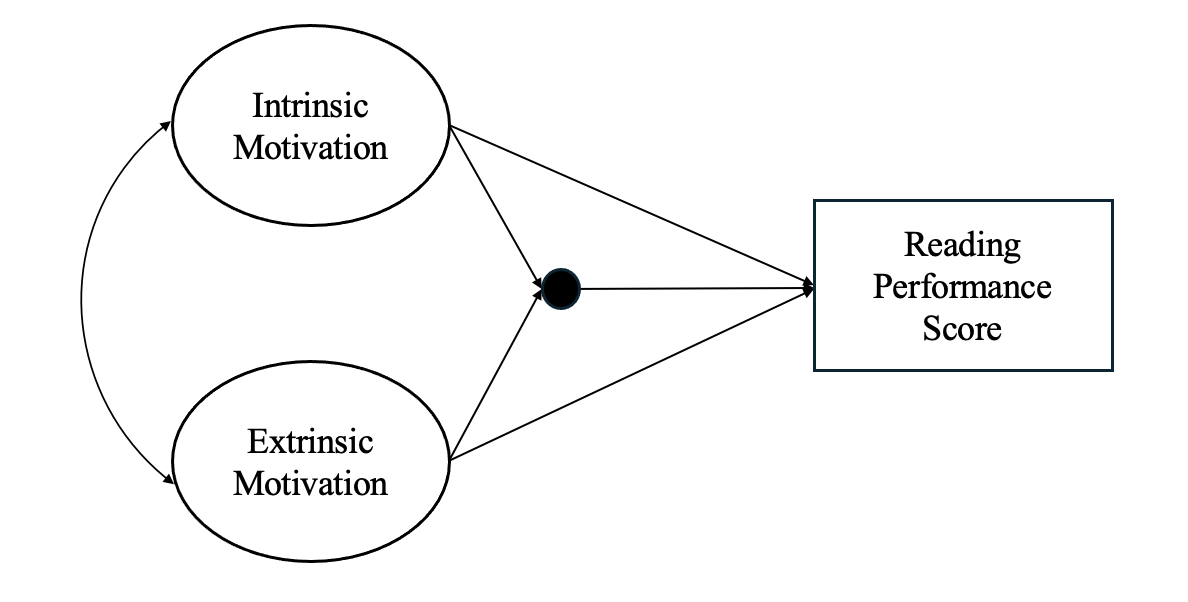
\includegraphics[width=0.8\textwidth]{/Users/jimmy_z/R Projects/2SPA-Int/Paper/Qual 1 Paper Draft/PIRL_Plot.png}
\caption{Structural Model of Illustrative Example from Park (2011).}
\caption*{\textit{Note. The model includes two first-order latent variables, intrinsic motivation and extrinsic motivation, depicted as ellipses. Their latent interaction term was depicted as a filled black circle. The dependent variable was observed and rendered as a rectangle.}}
\end{figure}

\section{Discussion}\label{discussion}

Applied researchers often explore complex relationships between variables, such as interactions. However, classical regression models, which assume that variables are free from measurement error, have been shown to yield biased estimates. As a result, latent variable approaches within the SEM framework are gaining prominence. In this study, we reviewed and compared the performance of three latent interaction methods (matched-pair UPI, RAPI, and 2S-PA-Int) in estimating interaction effects on congeneric items with varying factor loadings and measurement errors. Additionally, the regression-based approach using observed indicators, MMR, was included as a reference method.

We extended the 2S-PA model by Lai and Hsiao (2022) to support latent interaction estimation, namely 2S-PA-Int. The primary distinction between matched-pair UPI, RAPI, and 2S-PA-Int lies in the formation of latent interaction term. Matched-pair UPI constructs the interaction term using multiple product indicators (PIs) generated from first-order indicators, making it a multiple-indicator method. In contrast, RAPI and 2S-PA-Int use composite scores and factor scores as single indicators (SIs) for the interaction term, respectively.

Our results demonstrated that the MMR approach, based on observed indicators, consistently yielded substantially downward biased estimates of interaction effect path coefficients across multiple conditions. This finding can be attributed to the method's inefficiency to properly account for measurement errors in the observed items. The underestimated coefficients are consistent with previous research, which has emphasized that measurement error might result in biased parameter estimates (Dunlap \& Kemery, 1988; Evans, 1985).

In contrast, the latent interaction methods were effective in producing unbiased estimates of interaction effects by accounting for measurement errors, as demonstrated in our simulation study. However, both RAPI and matched-pair UPI exhibited notably positive standardized bias (SB), suggesting a tendency to overestimate interaction effects when true effects were present. These findings aligned with previous research by Marsh et al. (2004), Hsiao et al. (2018), and Hsiao et al. (2021), which similarly reported overestimation of interaction effects using matched-pair UPI and RAPI, particularly when dealing with congeneric items or tau-equivalent items with varied error variances. 2S-PA-Int also showed a tendency to overestimate interaction effects, further emphasizing that latent interaction methods should be applied carefully and cautiously, especially when more conservative estimates are needed. In terms of accuracy in estimating interaction effects, 2S-PA-Int demonstrates comparability to other latent interaction methods and presents a more reliable alternative to MMR when estimating interaction effects using congeneric items with measurement error.

One challenge in using latent variable modeling approaches for interaction effects is the risk of generating unstable estimates across replications, as reflected by the convergence rates and relative standard error (SE) estimates in the simulation results. In some cases, extreme SE estimates reaching values as high as 200 were observed, which is neither reasonable nor appropriate for coefficient interpretation and model comparison. This finding is consistent with previous research by Hsiao et al. (2021) and Ledgerwood and Shrout (2011), such that while latent interaction models improve accuracy by accounting for measurement error, they can also introduce increased variability in parameter estimates. Besides, Hsiao et al. (2018) noted that constraining measurement errors for highly reliable variables may lead to over-adjustment of SE, particularly with small sample sizes. Our RMSE results supported this finding, such that latent interaction methods generally exhibited higher RMSE values compared to MMR when the sample size was 100. Consequently, a latent variable model that can simultaneously yield both accurate and stable estimation should be recommended. Although all three latent interaction methods in our simulation study showed unacceptable relative SE bias in some small sample size and low reliability conditions, 2S-PA-Int generally demonstrates comparable stability in estimating interaction effects. In addition, 2S-PA-Int among the latent interaction methods produced the lowest RMSE values that were nearly comparable to those of MMR, which further supports that it has potential of taking into account accuracy and variability of parameter estimation.

With respect to coverage rates, RAPI showed notably higher coverage rates than matched-pair UPI and 2S-PA-Int, which can be partially attributed to its inflated SE estimation. While slightly lower, 2S-PA-Int also achieved acceptable coverage rates over 93\%, suggesting its capacity for capturing true interaction effects reliably. The results imply that both RAPI and 2S-PA-Int possess sufficient capability of effectively detecting interaction effects across varied conditions. In contrast, matched-pair UPI is not consistently robust to small sample sizes and low reliability levels. The observation is aligned with Marsh et al. (2004), although it should be noted that Marsh et al. (2004) did not evaluate matched-pair UPI with fully congeneric items, which may partly explain its reduced ability to capture true effects under such conditions. By ignoring measurement error, MMR failed to show sufficient coverage rates across almost all conditions, indicating that in general it could not capture true interaction effects. One possible reason is that downward SE estimates of MMR result in narrower confidence intervals, which increases the likelihood of missing true effects.

Revisiting Marsh's criteria for an effective latent interaction model, 2S-PA-Int stands out for its simplicity as a single-indicator method and its efficient use of information through factor scores based on all first-order indicators. Models burdened with excessive indicators often face convergence issues due to complex covariance structures, potentially resulting in non-identifiable models (Bollen, 1989). Moreover, Byrne (2016) points out that too many indicators can introduce redundancy, unnecessarily complicating the model and increasing the risk of estimation problems. Therefore, 2S-PA-Int emerges as a good alternative to matched-pair UPI in terms of simpler model and stable parameter estimation, especially with a large number of first-order indicators. Compared to RAPI, 2S-PA-Int also offers greater stability and accuracy in estimating interaction effects. Overall, latent interaction methods for composite scores are preferable to MMR when considering both precision and bias in the estimation of interaction effect, with 2S-PA-Int demonstrating the greatest potential among the methods.

While 2S-PA-Int demonstrated promising statistical properties in our simulation study, it is important to recognize several limitations in the limited scope of study design. First, given that the study focused exclusively on product indicator (PI) methods, distribution-analytic approaches such as the latent moderated structural equation (LMS; Klein \& Moosbrugger, 2000) method, and other alternative methods, were not included. Previous research has shown that LMS tends to produce unbiased estimates of latent interaction effects with acceptable statistical power when applied to congeneric items with normal distributions (Cham et al., 2012; Hsiao et al., 2021). Future studies can incorporate more alternative methods of estimating latent interaction effects to expand the scope of study.

Second, with regard to method application, we do not recommend the use of 2S-PA-Int for extreme cases where the sample size is less than 100 and item reliability falls below 0.7. Additionally, as Hsiao et al. (2018) noted, RAPI may be more practical for researchers working with secondary datasets, where only composite scores and their corresponding reliability indices (e.g., Cronbach's alpha) are typically available. In such cases, when factor scores and their standard errors are not provided, researchers may be unable to compute factor scores, thereby limiting the feasibility of applying 2S-PA-Int. Furthermore, the present study focused on congeneric items that were continuous and normally distributed. However, much research has highlighted the frequent use of categorical data in psychological studies to assess qualitative dimensions of human behavior, attitudes, and traits (Brown, 2015; Kline, 2016). Despite the lack of evaluation of 2S-PA-Int with categorical items in this study, its ability to incorporate observation-specific standard errors of measurement suggests that it may be well-suited for estimating latent interaction effects with categorical data in future research (Lai et al., 2023).

Additionally, previous research on latent interaction effects has typically employed simplified designs with two latent predictors and a single interaction term, which may not adequately reflect the complexity of real-world scenarios that involve multiple interaction terms. Given the increasing prevalence of multilevel designs in educational, counseling, and organizational research (e.g., students nested within classrooms, patients within clinics, employees within companies), it is important to investigate the applicability of 2S-PA-Int in handling more complex data structures. Future research could explore how 2S-PA-Int performs in multilevel contexts, particularly under varying sample sizes and reliability levels, to assess its robustness and versatility in such advanced analytical frameworks.

\newpage

\section{References}\label{references}

\phantomsection\label{refs}
\begin{CSLReferences}{1}{0}
\bibitem[\citeproctext]{ref-alginaNoteEstimatingJoreskogYang2001}
Algina, J., \& Moulder, B. C. (2001). A note on estimating the {J{ö}reskog-Yang} model for latent variable interaction using {LISREL} 8.3. \emph{Structural Equation Modeling}, \emph{8}(1), 40--52. \url{https://doi.org/10.1207/S15328007SEM0801_3}

\bibitem[\citeproctext]{ref-andersonComparisonBiasMean1996}
Anderson, L. E., Stone-Romero, E. F., \& Tisak, J. (1996). A {Comparison} of bias and mean squared error in parameter estimates of interaction effects: {Moderated} multiple regression versus error-in-variables regression. \emph{Multivariate Behavioral Research}, \emph{31}(1), 69--94. \url{https://doi.org/10.1207/s15327906mbr3101_5}

\bibitem[\citeproctext]{ref-bollenStructuralEquationsLatent1989d}
Bollen, K. A. (1989). \emph{Structural equations with latent variables} (pp. xiv, 514). John Wiley \& Sons. \url{https://doi.org/10.1002/9781118619179}

\bibitem[\citeproctext]{ref-bollenLatentVariablesPsychology2002a}
Bollen, K. A. (2002). Latent variables in psychology and the social sciences. \emph{Annual Review of Psychology}, \emph{53}(1), 605--634. \url{https://doi.org/10.1146/annurev.psych.53.100901.135239}

\bibitem[\citeproctext]{ref-bollenTestingStructuralEquation1993}
Bollen, K. A., \& Long, J. S. (Eds.). (1993). \emph{Testing structural equation models} (p. 320). Sage Publications, Inc.

\bibitem[\citeproctext]{ref-bradleyRobustness1978}
Bradley, J. V. (1978). Robustness? \emph{British Journal of Mathematical and Statistical Psychology}, \emph{31}(2), 144--152. \url{https://doi.org/10.1111/j.2044-8317.1978.tb00581.x}

\bibitem[\citeproctext]{ref-brownConfirmatoryFactorAnalysis2015b}
Brown, T. A. (2015). \emph{Confirmatory factor analysis for applied research, 2nd ed} (pp. xvii, 462). The Guilford Press.

\bibitem[\citeproctext]{ref-browneAlternativeWaysAssessing1992}
Browne, M. W., \& Cudeck, R. (1992). Alternative ways of assessing model fit. \emph{Sociological Methods \& Research}, \emph{21}(2), 230--258. \url{https://doi.org/10.1177/0049124192021002005}

\bibitem[\citeproctext]{ref-byrneStructuralEquationModeling2016}
Byrne, B. M. (2016). \emph{Structural equation modeling with {AMOS}: {Basic} concepts, applications, and programming} (3rd ed.). Routledge. \url{https://doi.org/10.4324/9781315757421}

\bibitem[\citeproctext]{ref-carrollMeasurementErrorNonlinear2006}
Carroll, R. J., Ruppert, D., Stefanski, L. A., \& Crainiceanu, C. M. (2006). \emph{Measurement error in nonlinear models: {A} modern perspective, second edition} (2nd ed.). {Chapman and Hall/CRC}. \url{https://doi.org/10.1201/9781420010138}

\bibitem[\citeproctext]{ref-cartePursuitModerationNine2003b}
Carte, T. A., \& Russell, C. J. (2003). In pursuit of moderation: {Nine} common errors and their solutions. \emph{MIS Quarterly}, \emph{27}(3), 479--501. \url{https://doi.org/10.2307/30036541}

\bibitem[\citeproctext]{ref-chamEstimatingLatentVariable2012a}
Cham, H., West, S. G., Ma, Y., \& Aiken, L. S. (2012). Estimating latent variable interactions with non-normal observed data: {A} comparison of four approaches. \emph{Multivariate Behav Res}, \emph{47}(6), 840--876. \url{https://doi.org/10.1080/00273171.2012.732901}

\bibitem[\citeproctext]{ref-chinPartialLeastSquares2003}
Chin, W. W., Marcolin, B. L., \& Newsted, P. R. (2003). A partial least squares latent variable modeling approach for measuring interaction effects: {Results} from a {Monte Carlo} simulation study and an electronic-mail emotion/adoption study. \emph{Information Systems Research}, \emph{14}(2), 189--217. \url{https://doi.org/10.1287/isre.14.2.189.16018}

\bibitem[\citeproctext]{ref-cohenAppliedMultipleRegression2003}
Cohen, J., Cohen, P., West, S. G., \& Aiken, L. S. (2003). \emph{Applied multiple regression/correlation analysis for the behavioral sciences, 3rd ed} (pp. xxviii, 703). Lawrence Erlbaum Associates Publishers.

\bibitem[\citeproctext]{ref-collinsComparisonInclusiveRestrictive2001}
Collins, L. M., Schafer, J. L., \& Kam, C. M. (2001). \href{https://www.ncbi.nlm.nih.gov/pubmed/11778676}{A comparison of inclusive and restrictive strategies in modern missing data procedures}. \emph{Psychol Methods}, \emph{6}(4), 330--351.

\bibitem[\citeproctext]{ref-cronbachCoefficientAlphaInternal1951}
Cronbach, L. J. (1951). Coefficient alpha and the internal structure of tests. \emph{Psychometrika}, \emph{16}(3), 297--334. \url{https://doi.org/10.1007/BF02310555}

\bibitem[\citeproctext]{ref-cunninghamModerationSportManagement2019a}
Cunningham, G. B., \& Ahn, N. Y. (2019). Moderation in sport management research: {Room} for growth. \emph{Measurement in Physical Education and Exercise Science}, \emph{23}(4), 301--313. \url{https://doi.org/10.1080/1091367X.2018.1472095}

\bibitem[\citeproctext]{ref-daszykowskiRobustStatisticsData2007}
Daszykowski, M., Kaczmarek, K., Vander Heyden, Y., \& Walczak, B. (2007). Robust statistics in data analysis --- {A} review. \emph{Chemometrics and Intelligent Laboratory Systems}, \emph{85}(2), 203--219. \url{https://doi.org/10.1016/j.chemolab.2006.06.016}

\bibitem[\citeproctext]{ref-dejonckereUsingBoundedEstimation2022}
De Jonckere, J., \& Rosseel, Y. (2022). Using {Bounded Estimation} to {Avoid Nonconvergence} in {Small Sample Structural Equation Modeling}. \emph{Structural Equation Modeling: A Multidisciplinary Journal}, \emph{29}(3), 412--427. \url{https://doi.org/10.1080/10705511.2021.1982716}

\bibitem[\citeproctext]{ref-dekkingModernIntroductionProbability2005a}
Dekking, F. M., Kraaikamp, C., Lopuhaä, H. P., \& Meester, L. E. (2005). \emph{A {Modern Introduction} to {Probability} and {Statistics}}. Springer. \url{https://doi.org/10.1007/1-84628-168-7}

\bibitem[\citeproctext]{ref-devliegerHypothesisTestingUsing2016}
Devlieger, I., Mayer, A., \& Rosseel, Y. (2016). Hypothesis testing using factor score regression. \emph{Educ Psychol Meas}, \emph{76}(5), 741--770. \url{https://doi.org/10.1177/0013164415607618}

\bibitem[\citeproctext]{ref-dunlapEffectsPredictorIntercorrelations1988}
Dunlap, W. P., \& Kemery, E. R. (1988). Effects of predictor intercorrelations and reliabilities on moderated multiple regression. \emph{Organizational Behavior and Human Decision Processes}, \emph{41}(2), 248--258. \url{https://doi.org/10.1016/0749-5978(88)90029-5}

\bibitem[\citeproctext]{ref-estabrookComparisonFactorScore2013}
Estabrook, R., \& Neale, M. (2013). A comparison of factor score estimation methods in the presence of missing data: {Reliability} and an application to nicotine dependence. \emph{Multivariate Behav Res}, \emph{48}(1), 1--27. \url{https://doi.org/10.1080/00273171.2012.730072}

\bibitem[\citeproctext]{ref-evansMonteCarloStudy1985}
Evans, M. G. (1985). A {Monte Carlo} study of the effects of correlated method variance in moderated multiple regression analysis. \emph{Organizational Behavior and Human Decision Processes}, \emph{36}(3), 305--323. \url{https://doi.org/10.1016/0749-5978(85)90002-0}

\bibitem[\citeproctext]{ref-foldnesChoiceProductIndicators2014}
Foldnes, N., \& Hagtvet, K. A. (2014). The choice of product indicators in latent variable interaction models: {Post} hoc analyses. \emph{Psychological Methods}, \emph{19}(3), 444--457. \url{https://doi.org/10.1037/a0035728}

\bibitem[\citeproctext]{ref-hancockReliabilityAradoxAssessing2011}
Hancock, G. R., \& Mueller, R. O. (2011). The reliability aradox in assessing structural relations within covariance structure models. \emph{Educational and Psychological Measurement}, \emph{71}(2), 306--324. \url{https://doi.org/10.1177/0013164410384856}

\bibitem[\citeproctext]{ref-harwellStrategyUsingBias2019}
Harwell, M. (2019). A strategy for using bias and {RMSE} as outcomes in {Monte Carlo} studies in statistics. \emph{J. Mod. Appl. Stat. Methods}, \emph{17}(2), jmasm.eP2938. \url{https://doi.org/10.22237/jmasm/1551907966}

\bibitem[\citeproctext]{ref-hooglandRobustnessStudiesCovariance1998}
Hoogland, J. J., \& Boomsma, A. (1998). Robustness studies in covariance structure modeling: {An} overview and a meta-analysis. \emph{Sociological Methods \& Research}, \emph{26}(3), 329--367. \url{https://doi.org/10.1177/0049124198026003003}

\bibitem[\citeproctext]{ref-hsiaoEvaluationTwoMethods2018a}
Hsiao, Y.-Y., Kwok, O.-M., \& Lai, M. H. C. (2018). Evaluation of two methods for modeling measurement errors when testing interaction effects with observed composite scores. \emph{Educ Psychol Meas}, \emph{78}(2), 181--202. \url{https://doi.org/10.1177/0013164416679877}

\bibitem[\citeproctext]{ref-hsiaoModelingMeasurementErrors2021}
Hsiao, Y.-Y., Kwok, O.-M., \& Lai, M. H. C. (2021). Modeling measurement errors of the exogenous composites from congeneric measures in interaction models. \emph{Struct Equ Modeling}, \emph{28}(2), 250--260. \url{https://doi.org/10.1080/10705511.2020.1782206}

\bibitem[\citeproctext]{ref-huCutoffCriteriaFit1999}
Hu, L., \& Bentler, P. M. (1999). Cutoff criteria for fit indexes in covariance structure analysis: {Conventional} criteria versus new alternatives. \emph{Structural Equation Modeling}, \emph{6}(1), 1--55. \url{https://doi.org/10.1080/10705519909540118}

\bibitem[\citeproctext]{ref-huberRobustStatistics2011}
Huber, P. J. (2011). Robust {Statistics}. In M. Lovric (Ed.), \emph{International {Encyclopedia} of {Statistical Science}} (pp. 1248--1251). Springer. \url{https://doi.org/10.1007/978-3-642-04898-2_594}

\bibitem[\citeproctext]{ref-jackmanEstimatingLatentVariable2011a}
Jackman, G.-A., Leite, W., \& Cochrane, D. (2011). Estimating latent variable interactions with the unconstrained approach: {A} comparison of methods to form product indicators for large, unequal numbers of items. \emph{Structural Equation Modeling}, \emph{18}, 274--288. \url{https://doi.org/10.1080/10705511.2011.557342}

\bibitem[\citeproctext]{ref-joreskogStatisticalAnalysisSets1971}
Jöreskog, K. G. (1971). Statistical analysis of sets of congeneric tests. \emph{Psychometrika}, \emph{36}(2), 109--133. \url{https://doi.org/10.1007/BF02291393}

\bibitem[\citeproctext]{ref-joreskogLISRELStructuralEquation1993}
Jöreskog, K. G., \& Sörbom, D. (1993). \emph{{LISREL} 8: {Structural} equation modeling with the {SIMPLIS} command language} (pp. xvi, 202). Lawrence Erlbaum Associates, Inc.

\bibitem[\citeproctext]{ref-Jreskog1996NonlinearSE}
Jöreskog, K. G., \& Yang, F. (1996). \emph{Nonlinear structural equation models: {The Kenny-Judd} model with {Interaction} effects}.

\bibitem[\citeproctext]{ref-kennyEstimatingNonlinearInteractive1984a}
Kenny, D. A., \& Judd, C. M. (1984). Estimating the nonlinear and interactive effects of latent variables. \emph{Psychological Bulletin}, \emph{96}(1), 201--210. \url{https://doi.org/10.1037/0033-2909.96.1.201}

\bibitem[\citeproctext]{ref-kleinMaximumLikelihoodEstimation2000a}
Klein, A., \& Moosbrugger, H. (2000). Maximum likelihood estimation of latent interaction effects with the {LMS} method. \emph{Psychometrika}, \emph{65}(4), 457--474. \url{https://doi.org/10.1007/BF02296338}

\bibitem[\citeproctext]{ref-klinePrinciplesPracticeStructural2016}
Kline, R. B. (2016). \emph{Principles and practice of structural equation modeling, 4th ed} (pp. xvii, 534). Guilford Press.

\bibitem[\citeproctext]{ref-kyriazosAppliedPsychometricsSample2018}
Kyriazos, T. (2018). Applied psychometrics: {Sample} size and sample power considerations in factor analysis ({EFA}, {CFA}) and {SEM} in general. \emph{Psychology}, \emph{09}, 2207--2230. \url{https://doi.org/10.4236/psych.2018.98126}

\bibitem[\citeproctext]{ref-laiTwostagePathAnalysis2022a}
Lai, M. H. C., \& Hsiao, Y.-Y. (2022). Two-stage path analysis with definition variables: {An} alternative framework to account for measurement error. \emph{Psychological Methods}, \emph{27}(4), 568--588. \url{https://doi.org/10.1037/met0000410}

\bibitem[\citeproctext]{ref-laiCorrectingUnreliabilityPartial2023}
Lai, M. H. C., Tse, W. W.-Y., Zhang, G., Li, Y., \& Hsiao, Y.-Y. (2023). Correcting for unreliability and partial invariance: {A} two-stage path analysis approach. \emph{Structural Equation Modeling: A Multidisciplinary Journal}, \emph{30}(2), 258--271. \url{https://doi.org/10.1080/10705511.2022.2125397}

\bibitem[\citeproctext]{ref-ledgerwoodTradeaccuracyPrecisionLatent2011}
Ledgerwood, A., \& Shrout, P. E. (2011). The trade-off between accuracy and precision in latent variable models of mediation processes. \emph{Journal of Personality and Social Psychology}, \emph{101}(6), 1174--1188. \url{https://doi.org/10.1037/a0024776}

\bibitem[\citeproctext]{ref-linStructuralEquationModels2010b}
Lin, G.-C., Wen, Z., Marsh, H. W., \& Lin, H.-S. (2010). Structural equation models of latent interactions: {Clarification} of orthogonalizing and double-mean-centering strategies. \emph{Structural Equation Modeling: A Multidisciplinary Journal}, \emph{17}(3), 374--391. \url{https://doi.org/10.1080/10705511.2010.488999}

\bibitem[\citeproctext]{ref-lordStatisticalTheoriesMental1968}
Lord, F. M., Novick, M. R., \& Birnbaum, A. (1968). \emph{Statistical theories of mental test scores}. Addison-Wesley.

\bibitem[\citeproctext]{ref-mackinnonHowWhomMediation2008a}
MacKinnon, D. P., \& Luecken, L. J. (2008). How and for whom? {Mediation} and moderation in health psychology. \emph{Health Psychol}, \emph{27}(2S), S99--S100. \url{https://doi.org/10.1037/0278-6133.27.2(Suppl.).S99}

\bibitem[\citeproctext]{ref-marshStructuralEquationModels2004a}
Marsh, H. W., Wen, Z., \& Hau, K.-T. (2004). Structural equation models of latent interactions: Evaluation of alternative estimation strategies and indicator construction. \emph{Psychol Methods}, \emph{9}(3), 275--300. \url{https://doi.org/10.1037/1082-989X.9.3.275}

\bibitem[\citeproctext]{ref-maslowskyEstimatingInterpretingLatent2015a}
Maslowsky, J., Jager, J., \& Hemken, D. (2015). Estimating and interpreting latent variable interactions: {A} tutorial for applying the latent moderated structural equations method. \emph{Int J Behav Dev}, \emph{39}(1), 87--96. \url{https://doi.org/10.1177/0165025414552301}

\bibitem[\citeproctext]{ref-mcdonaldTheoreticalFoundationsPrincipal1970}
McDonald, R. P. (1970). The theoretical foundations of principal factor analysis, canonical factor analysis, and alpha factor analysis. \emph{British Journal of Mathematical and Statistical Psychology}, \emph{23}(1), 1--21. \url{https://doi.org/10.1111/j.2044-8317.1970.tb00432.x}

\bibitem[\citeproctext]{ref-moulderComparisonMethodsEstimating2002a}
Moulder, B. C., \& Algina, J. (2002). Comparison of methods for estimating and testing latent variable interactions. \emph{Structural Equation Modeling}, \emph{9}(1), 1--19. \url{https://doi.org/10.1207/S15328007SEM0901_1}

\bibitem[\citeproctext]{ref-muellerStructuralEquationModeling1997a}
Mueller, R. O. (1997). Structural equation modeling: {Back} to basics. \emph{Structural Equation Modeling}, \emph{4}(4), 353--369. \url{https://doi.org/10.1080/10705519709540081}

\bibitem[\citeproctext]{ref-mvffrw23}
Mullis, I. V. S., von Davier, Matthias, Foy, P., Fishbein, B., Reynolds, K. A., \& Wry, E. (2023). \emph{PIRLS 2021 international results in reading}. Boston College.

\bibitem[\citeproctext]{ref-mullisPIRLS2006International2007}
Mullis, I., Martin, M., \& Foy, P. (2007). \emph{{PIRLS} 2006 international report: {IEA}'s {Progress} in {International Reading Literacy Study} in primary schools in 40 countries}. Chestnut Hill, MA : Boston College.

\bibitem[\citeproctext]{ref-muthenHowUseMonte2002}
Muthén, L. K., \& Muthén, B. O. (2002). How to use a {Monte Carlo} study to decide on sample size and determine power. \emph{Structural Equation Modeling: A Multidisciplinary Journal}, \emph{9}(4), 599--620. \url{https://doi.org/10.1207/S15328007SEM0904_8}

\bibitem[\citeproctext]{ref-parkHowMotivationalConstructs2011}
Park, Y. (2011). How motivational constructs interact to predict elementary students' reading performance: {Examples} from attitudes and self-concept in reading. \emph{Learning and Individual Differences}, \emph{21}(4), 347--358. \url{https://doi.org/10.1016/j.lindif.2011.02.009}

\bibitem[\citeproctext]{ref-radloffCESDScaleSelfreport1977b}
Radloff, L. S. (1977). The {CES-D} scale: {A} self-report depression scale for research in the general population. \emph{Applied Psychological Measurement}, \emph{1}(3), 385--401. \url{https://doi.org/10.1177/014662167700100306}

\bibitem[\citeproctext]{ref-raykovEstimationCompositeReliability1997}
Raykov, T. (1997). Estimation of composite reliability for congeneric measures. \emph{Applied Psychological Measurement}, \emph{21}(2), 173--184. \url{https://doi.org/10.1177/01466216970212006}

\bibitem[\citeproctext]{ref-rosseel2012}
Rosseel, Y. (2012). {lavaan}: An {R} package for structural equation modeling. \emph{Journal of Statistical Software}, \emph{48}(2), 1--36. \url{https://doi.org/10.18637/jss.v048.i02}

\bibitem[\citeproctext]{ref-rousseeuwAlternativesMedianAbsolute1993}
Rousseeuw, P. J., \& Croux, C. (1993). Alternatives to the {Median Absolute Deviation}. \emph{Journal of the American Statistical Association}, \emph{88}(424), 1273--1283. \url{https://doi.org/10.2307/2291267}

\bibitem[\citeproctext]{ref-rousseeuwRobustStatisticsOutlier2011}
Rousseeuw, P. J., \& Hubert, M. (2011). Robust statistics for outlier detection. \emph{WIREs Data Mining and Knowledge Discovery}, \emph{1}(1), 73--79. \url{https://doi.org/10.1002/widm.2}

\bibitem[\citeproctext]{ref-schoemannTestingInterpretingLatent2021}
Schoemann, A. M., \& Jorgensen, T. D. (2021). Testing and interpreting latent variable interactions using the {semTools} package. \emph{Psych}, \emph{3}(3), 322--335. \url{https://doi.org/10.3390/psych3030024}

\bibitem[\citeproctext]{ref-steinmetzThreeApproachesEstimate2011a}
Steinmetz, H., Davidov, E., \& Schmidt, P. (2011). Three approaches to estimate latent interaction effects: {Intention} and perceived behavioral control in the theory of planned behavior. \emph{Methodological Innovations Online}, \emph{6}(1), 95--110. \url{https://doi.org/10.4256/mio.2010.0030}

\bibitem[\citeproctext]{ref-tenbergeGreatestLowerBound2004}
Ten Berge, J. M. F., \& Sočan, G. (2004). The greatest lower bound to the reliability of a test and the hypothesis of unidimensionality. \emph{Psychometrika}, \emph{69}(4), 613--625. \url{https://doi.org/10.1007/BF02289858}

\bibitem[\citeproctext]{ref-vmff23}
von Davier, M., Mullis, I. V. S., Fishbein, B., \& Foy, P. (Eds.). (2023). \emph{Methods and procedures: PIRLS 2021 technical report}. Boston College, TIMSS \& PIRLS International Study Center. \url{https://pirls2021.org/methods}

\bibitem[\citeproctext]{ref-wuComparisonStrategiesForming2013}
Wu, Y., Wen, Z., Marsh, H., \& Hau, K.-T. (2013). A comparison of strategies for forming product indicators for unequal numbers of items in structural equation models of latent interactions. \emph{Structural Equation Modeling: A Multidisciplinary Journal}, \emph{20}, 551--567. \url{https://doi.org/10.1080/10705511.2013.824772}

\end{CSLReferences}


\end{document}
